\documentclass[amssymb,amsmath]{beamer}
\usetheme{Boadilla}
%\usepackage[english]{babel}
\usepackage{graphicx}
\usepackage{wrapfig}
\usepackage{color}
\usepackage{multicol}
\usepackage{tikz}
%%%%%%%%%%%%%%%
\usepackage{bookmath} % definitions and shortcuts
%%%%%%%%%%%%%%%
\setbeamertemplate{frametitle}{ \bf
\begin{centering} 
\insertframetitle 
\par 
\end{centering} 
}
%%%%%%%%%%%%%%%% 
\newcommand{\cecoin}{CeCoIn$_5$} 
\newcommand{\kbtf}{$\kappa$-(BEDT-TTF)$_2$Cu(NCS)$_2$}
\newcommand{\black}{\textcolor{black}}
\newcommand{\blue}{\textcolor{blue}}
\newcommand{\red}{\textcolor{red}}
\newcommand{\green}{\textcolor{green}}
\newcommand{\olive}{\textcolor{olive}}
\newcommand\Fontvi{\fontsize{9}{9}\selectfont}
\newcommand\Fontvii{\fontsize{4}{4}\selectfont}
\newcommand\Fontv{\fontsize{11}{11}\selectfont}
\newcommand\Fontb{\fontsize{15}{15}\selectfont}
\newcommand\Fontsm{\fontsize{13}{13}\selectfont}
%%%%%%%%%%%%%%%%%%%%%%%%%%%%%%%%%%%%%%%%%%%%%%%%%%%%%%%
%%%%%%%%%%%%%%%%%%%%%%%%%%%%%%%%%%%%%%%%%%%%%%%%%%%%%%%

\title[non-uniform SC]{Non-uniform Superconductors and Magnetism}
\author[brosemeyer@physics.montana.edu]{Ben Rosemeyer \\ \small Advisor: Anton Vorontsov}
\institute[MSU]{

\includegraphics[scale=0.2]{./figures/MSUlogo.jpg}\\[0.5cm]
Funded by NSF grant DMR-0954342 \\

\includegraphics[scale=0.08]{./figures/NSFlogo.jpg}
}
\date[CAM 2015]{\small\today}



\begin{document}
\frame{\titlepage}
%%%%%%%%%%%%%%%%%%%%%%%%%%%
\tikzstyle{every picture}+=[remember picture]
%%%%%%%%%%%%%%%%%%%%%%%%%%%
%\section*{Outline}
%\frame{\tableofcontents}

%%%%%%%%%%%%%%%%%%%%%%%%%%%%%%%%%%%%%%%%%%%%%%%%%%%%%%%%%%%%%%%%%%%%%%%%%%%%%%%%%%%%%%%%%%%%%%%%%%%%%%%%%%%%%%%%%%%%%%%%%%%%
%%%%%%%%%%%%%%%%%%%%%%%%%%%%%%%%%%%%%%%%%%%%%%%%%%%%%%%%%%%%%%%%%%%%%%%%%%%%%%%%%%%%%%%%%%%%%%%%%%%%%%%%%%%%%%%%%%%%%%%%%%%%
%%%%%%%%%%%%%%%%%%%%%%%%%%%%%%%%%%%%%%%%%%%%%%%%%%%%%%%%%%%%%%%%%%%%%%%%%%%%%%%%%%%%%%%%%%%%%%%%%%%%%%%%%%%%%%%%%%%%%%%%%%%%
\begin{frame}
\frametitle{What about a uniform superconductor???}
\centering
FORMATION OF ``COOPER PAIRS'' FROM ATTRACTION BETWEEN ELECTRONS WITH OPPOSITE MOMENTUM NEAR FS
 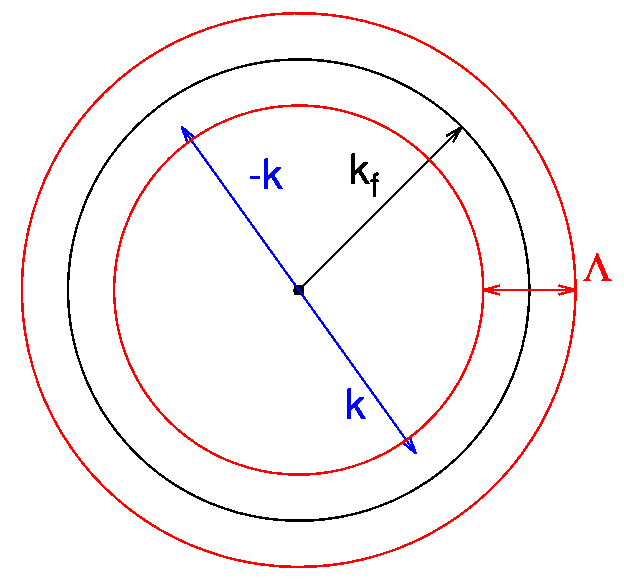
\includegraphics[scale=0.26]{./figures/Cooper_pairs.png}\\
MEAN FIELD HAMILTONIAN $\Rightarrow\,\,\cH_{\Delta} = \sum\limits_{\vk} \,\bigg[
    		\Delta_{\hk} a_{\vk\uparrow}^\dagger a_{-\vk\downarrow}^\dagger + h.c.\bigg]$ \\ 
BdG Transformation $\Rightarrow$\fbox{QUASI-PARTICLES = PARTICLE + HOLE}
\end{frame}
%%%%%%%%%%%%%%%%%%%%%%%%%%%%%%%%%%%%%%%%%%%%%%%%%%%%%%%%%%%%%%%%%%%%%%%%%%%%%%%%%%%%%%%%%%%%%%%%%%%%%%%%%%%%%%%%%%%%%%%%%%%%
%%%%%%%%%%%%%%%%%%%%%%%%%%%%%%%%%%%%%%%%%%%%%%%%%%%%%%%%%%%%%%%%%%%%%%%%%%%%%%%%%%%%%%%%%%%%%%%%%%%%%%%%%%%%%%%%%%%%%%%%%%%%
%%%%%%%%%%%%%%%%%%%%%%%%%%%%%%%%%%%%%%%%%%%%%%%%%%%%%%%%%%%%%%%%%%%%%%%%%%%%%%%%%%%%%%%%%%%%%%%%%%%%%%%%%%%%%%%%%%%%%%%%%%%%
\begin{frame}
\frametitle{What is a non-uniform superconductor???}
\centering
$\hat{y}$($\hat{x}$) momentum $\Rightarrow$ \fbox{GOOD(BAD)} quantum number \\$\Rightarrow \Delta(\vx,\vx') = \Delta(R_x)  \int d\vk \,\,\Delta_{\hk} e^{-i\vk\cdot\vr}\quad\quad \Delta_{\hk} = \{\red{1}, sin(2\theta_{\hk})\}$ \\
\centering
 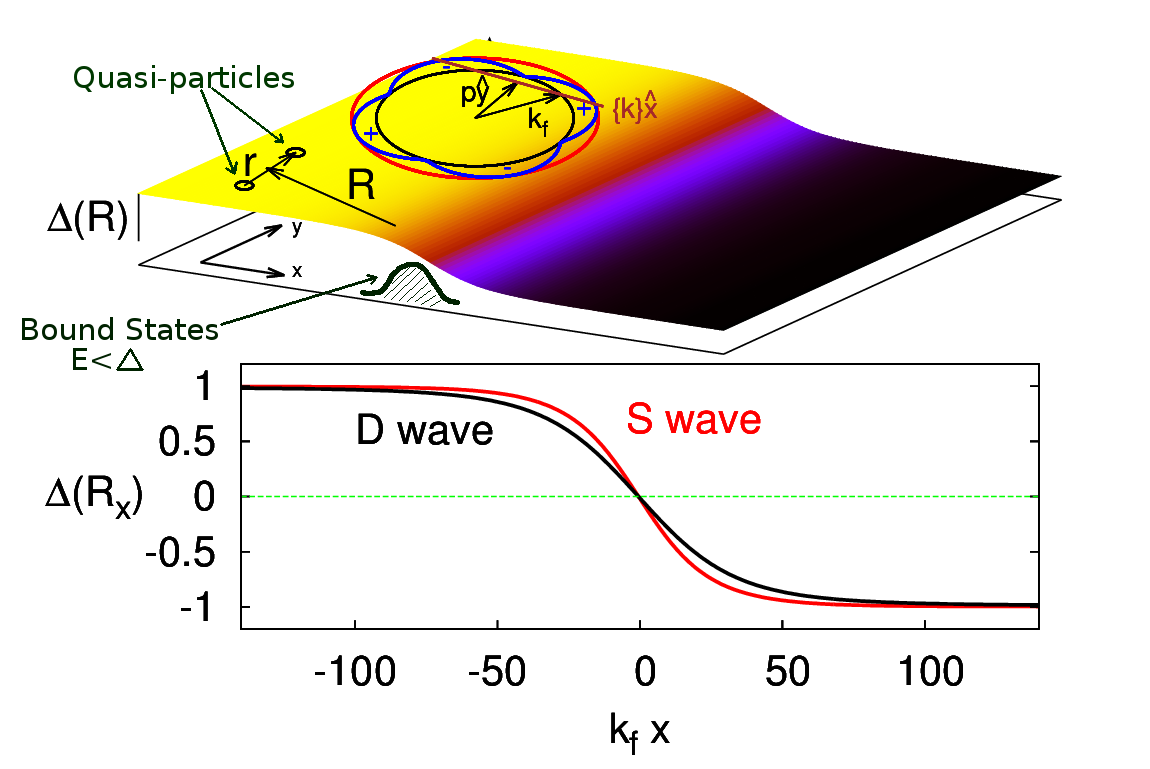
\includegraphics[scale=0.27]{./figures_3/fig1/Fig1_0.png}
\end{frame}
%%%%%%%%%%%%%%%%%%%%%%%%%%%%%%%%%%%%%%%%%%%%%%%%%%%%%%%%%%%%%%%%%%%%%%%%%%%%%%%%%%%%%%%%%%%%%%%%%%%%%%%%%%%%%%%%%%%%%%%%%%%%
%%%%%%%%%%%%%%%%%%%%%%%%%%%%%%%%%%%%%%%%%%%%%%%%%%%%%%%%%%%%%%%%%%%%%%%%%%%%%%%%%%%%%%%%%%%%%%%%%%%%%%%%%%%%%%%%%%%%%%%%%%%%
%%%%%%%%%%%%%%%%%%%%%%%%%%%%%%%%%%%%%%%%%%%%%%%%%%%%%%%%%%%%%%%%%%%%%%%%%%%%%%%%%%%%%%%%%%%%%%%%%%%%%%%%%%%%%%%%%%%%%%%%%%%%
\begin{frame}
\frametitle{Local Density of States}
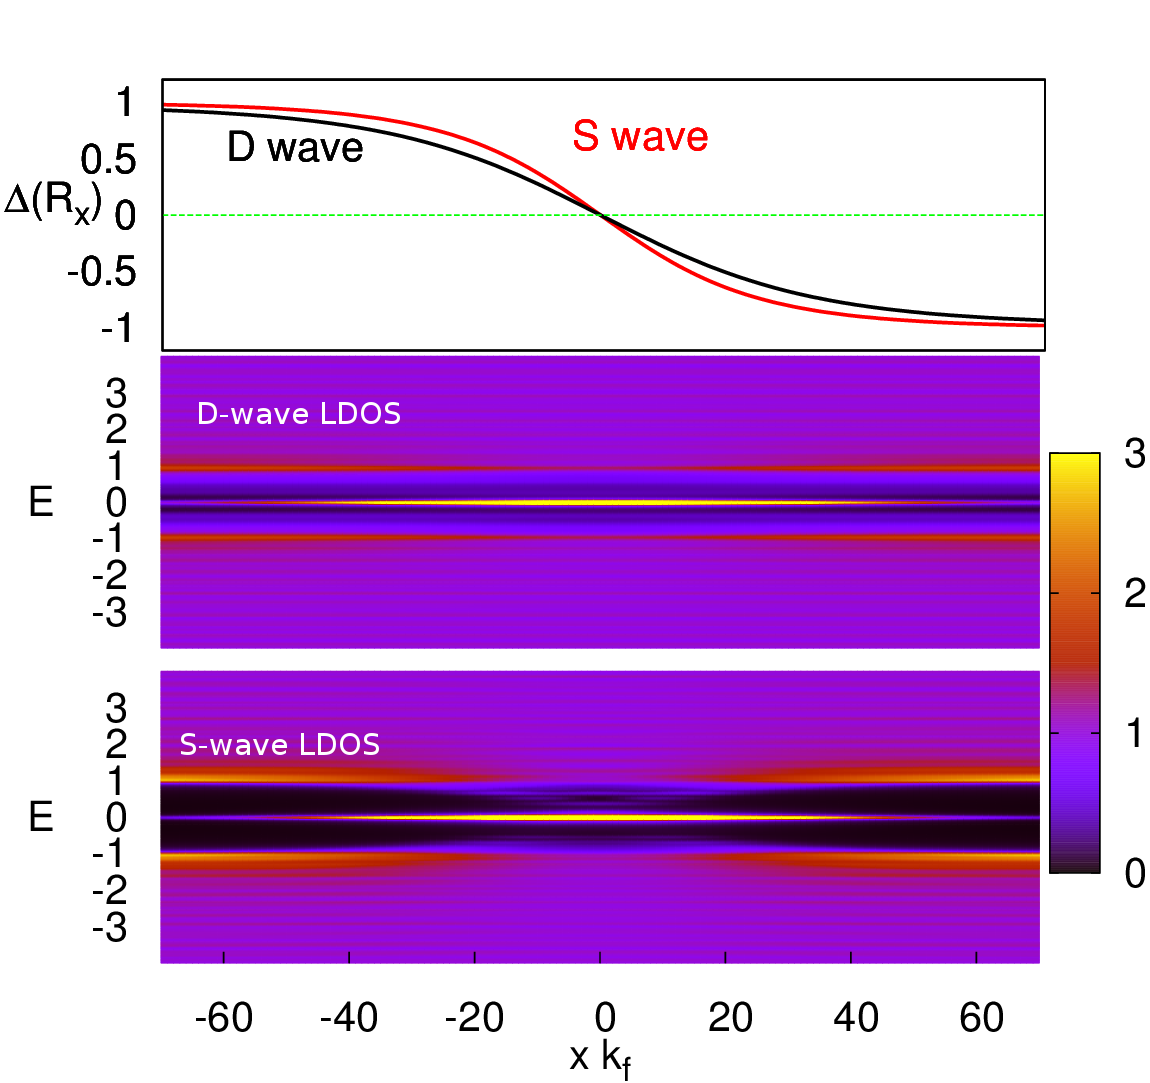
\includegraphics[scale=0.22]{./figures_3/fig1/Fig1.png}   
\end{frame}
%%%%%%%%%%%%%%%%%%%%%%%%%%%%%%%%%%%%%%%%%%%%%%%%%%%%%%%%%%%%%%%%%%%%%%%%%%%%%%%%%%%%%%%%%%%%%%%%%%%%%%%%%%%%%%%%%%%%%%%%%%%%
%%%%%%%%%%%%%%%%%%%%%%%%%%%%%%%%%%%%%%%%%%%%%%%%%%%%%%%%%%%%%%%%%%%%%%%%%%%%%%%%%%%%%%%%%%%%%%%%%%%%%%%%%%%%%%%%%%%%%%%%%%%%
%%%%%%%%%%%%%%%%%%%%%%%%%%%%%%%%%%%%%%%%%%%%%%%%%%%%%%%%%%%%%%%%%%%%%%%%%%%%%%%%%%%%%%%%%%%%%%%%%%%%%%%%%%%%%%%%%%%%%%%%%%%%
\begin{frame}
\frametitle{Question???}
\centering
{\huge How do bound states in a non-uniform superconductor affect \\
\blue{TRANSVERSE} magnetic properties?}\\
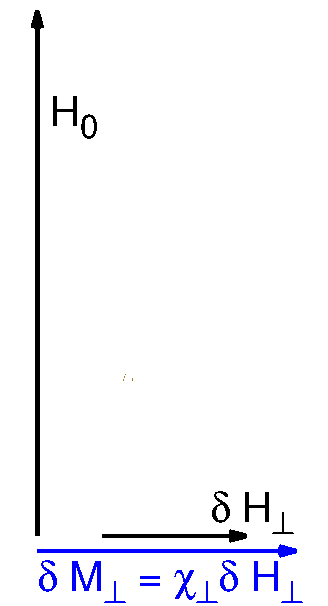
\includegraphics[scale=0.2]{./figures/Fig_field.png}
\hspace{0.1cm}
\fbox{\parbox[b]{0.39\linewidth}{
MAGNETIZATION \\\blue{$\delta M_{\perp}(\vq) = \bar{\chi}_{_\perp}(\vq)\delta H_{\perp}(\vq)$} \\
\vspace{0.5cm} \\HYPERFINE INT. \\ $\Rightarrow$RELAXATION RATE \\
$\Rightarrow\Rightarrow$NMR measurement
$T_{\perp}^{-1}$}}
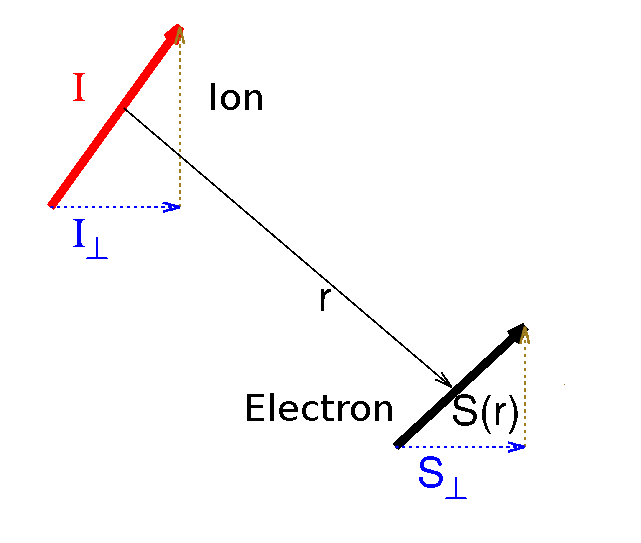
\includegraphics[scale=0.197]{./figures/Fig_rel_time.png}
\end{frame}

%%%%%%%%%%%%%%%%%%%%%%%%%%%%%%%%%%%%%%%%%%%%%%%%%%%%%%%%%%%%%%%%%%%%%%%%%%%%%%%%%%%%%%%%%%%%%%%%%%%%%%%%%%%%%%%%%%%%%%%%%%%%
%%%%%%%%%%%%%%%%%%%%%%%%%%%%%%%%%%%%%%%%%%%%%%%%%%%%%%%%%%%%%%%%%%%%%%%%%%%%%%%%%%%%%%%%%%%%%%%%%%%%%%%%%%%%%%%%%%%%%%%%%%%%
%%%%%%%%%%%%%%%%%%%%%%%%%%%%%%%%%%%%%%%%%%%%%%%%%%%%%%%%%%%%%%%%%%%%%%%%%%%%%%%%%%%%%%%%%%%%%%%%%%%%%%%%%%%%%%%%%%%%%%%%%%%%
\begin{frame} \frametitle{Motivation}

\begin{columns}
    \begin{column}{0.4\textwidth}
     	-FFLO\tikz\node[coordinate] (n1) {}; \\
     		{\Fontvii Burkhardt and Rainer (1994)} \\
    		-Vortex \tikz\node[coordinate] (n2) {}; \\
    			{\Fontvii Kakuyanagi et al. (2003)}\\
    		-Organic SCs \tikz\node[coordinate] (n3) {}; \\
    			{\Fontvii Mayaffre et al. (2014)}\\
    		-Topological States \tikz\node[coordinate] (n4) {}; \\
    			{\Fontvii Kashiwaya and Tanaka (2000)}\\
		\vspace{0.5cm}
	\tikz[baseline]{\node[anchor=base] (t4)
            {\frame{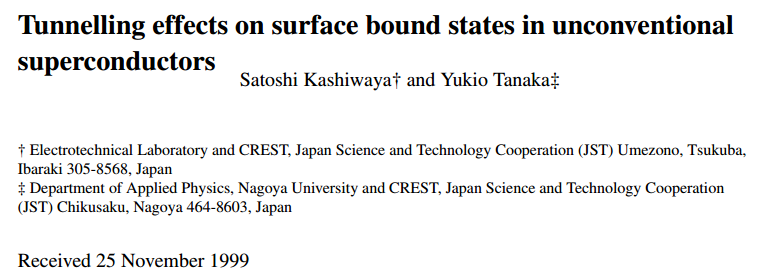
\includegraphics[scale=0.18]{./figures/unconventional_surface.png}}};}
    \end{column}
    \begin{column}{0.6\textwidth}
    \tikz[baseline]{\node[anchor=base] (t1)
            {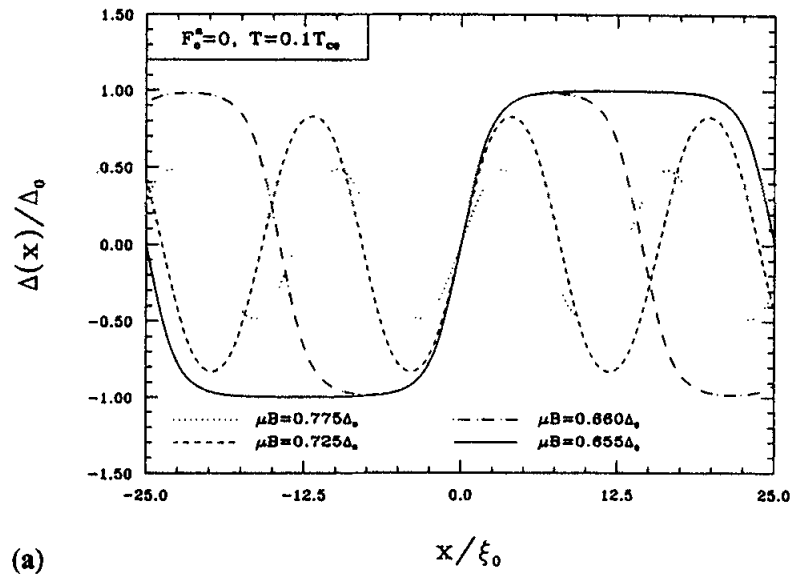
\includegraphics[scale=0.13]{./figures/Rainer_DW.png}};}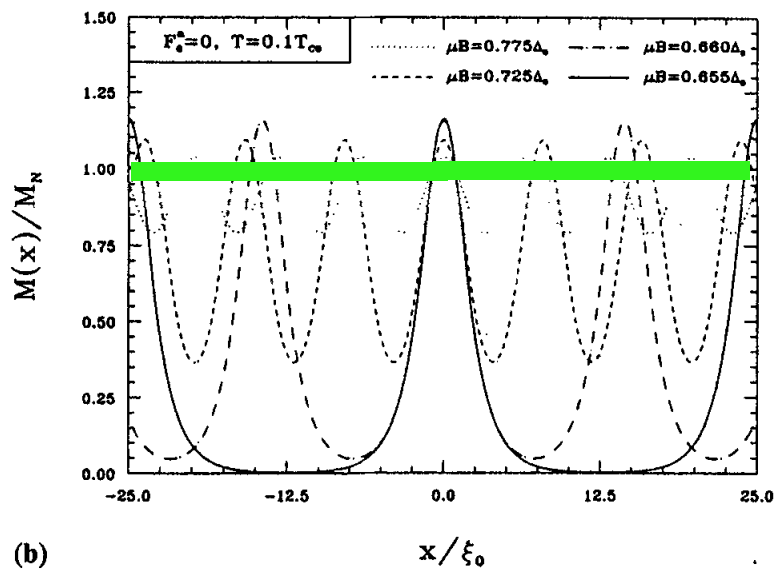
\includegraphics[scale=0.13]{./figures/Rainer_M.png} \\
    \tikz[baseline]{\node[anchor=base] (t2)
            {\frame{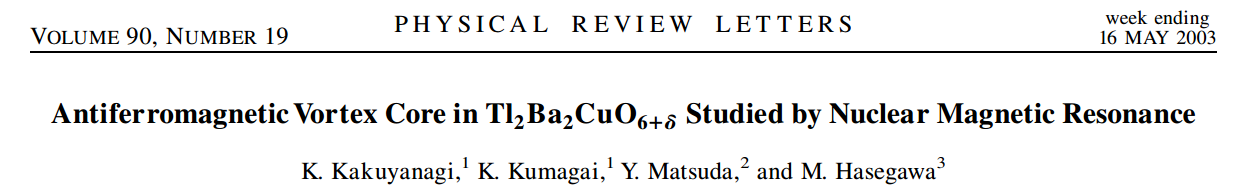
\includegraphics[scale=0.14]{./figures/AFM_vortex.png}}};} \\
    \tikz[baseline]{\node[anchor=base] (t3)
            {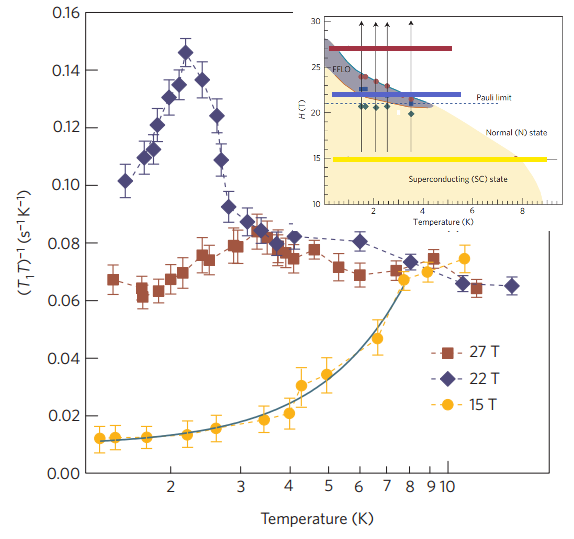
\includegraphics[scale=0.225]{./figures/organic_T1.png}};} \\
   
    \end{column}
  \end{columns}
   
\begin{tikzpicture}[overlay]
        \path[->]<1-> (n1) edge (t1);
        \path[->]<1-> (n2) edge (t2);
        \path[->]<1-> (n3) edge (t3);
        \path[->]<1-> (n4) edge (t4);
\end{tikzpicture}
\end{frame}

%%%%%%%%%%%%%%%%%%%%%%%%%%%%%%%%%%%%%%%%%%%%%%%%%%%%%%%%%%%%%%%%%%%%%%%%%%%%%%%%%%%%%%%%%%%%%%%%%%%%%%%%%%%%%%%%%%%%%%%%%%%%
%%%%%%%%%%%%%%%%%%%%%%%%%%%%%%%%%%%%%%%%%%%%%%%%%%%%%%%%%%%%%%%%%%%%%%%%%%%%%%%%%%%%%%%%%%%%%%%%%%%%%%%%%%%%%%%%%%%%%%%%%%%%
%%%%%%%%%%%%%%%%%%%%%%%%%%%%%%%%%%%%%%%%%%%%%%%%%%%%%%%%%%%%%%%%%%%%%%%%%%%%%%%%%%%%%%%%%%%%%%%%%%%%%%%%%%%%%%%%%%%%%%%%%%%%
\begin{frame} \frametitle{SUSCEPTIBILITY} 
PERTURBATION $\Rightarrow\,\,$ \fbox{$\cV = \mu_B\int d\vx \quad\Psi_\mu^\dagger(\vx,t) \vsigma_{\mu\nu}\cdot \delta \vH(\vx,t) \Psi_\nu(\vx,t)$} \\
$\chi_{_{\alpha\beta}}(\vx,\vx',\omega) = \frac{i\mu_B^2}{\chi_0}\int dt \quad e^{i\omega t}\langle [S_\alpha(\vx,t), S_\beta(\vx',0)]\theta(t) \rangle$ 
\begin{columns}
\begin{column}{0.42\textwidth}
$S_\alpha(\vx,t) = \Psi^\dagger_\mu(\vx,t) \sigma^{\alpha}_{\mu\nu}  \Psi^\dagger_\nu(\vx,t)$

\blue{\Fontvi $\Rightarrow$Transverse response \\\hspace{1cm}$(\alpha,\beta) = (x,x)\, or\, (y,y)$} \\

{\fbox{\red{$\chi(\vR,\vq) = \int d\vr e^{-i\vq\cdot\vr} \chi(\vR,\vr)$}}}

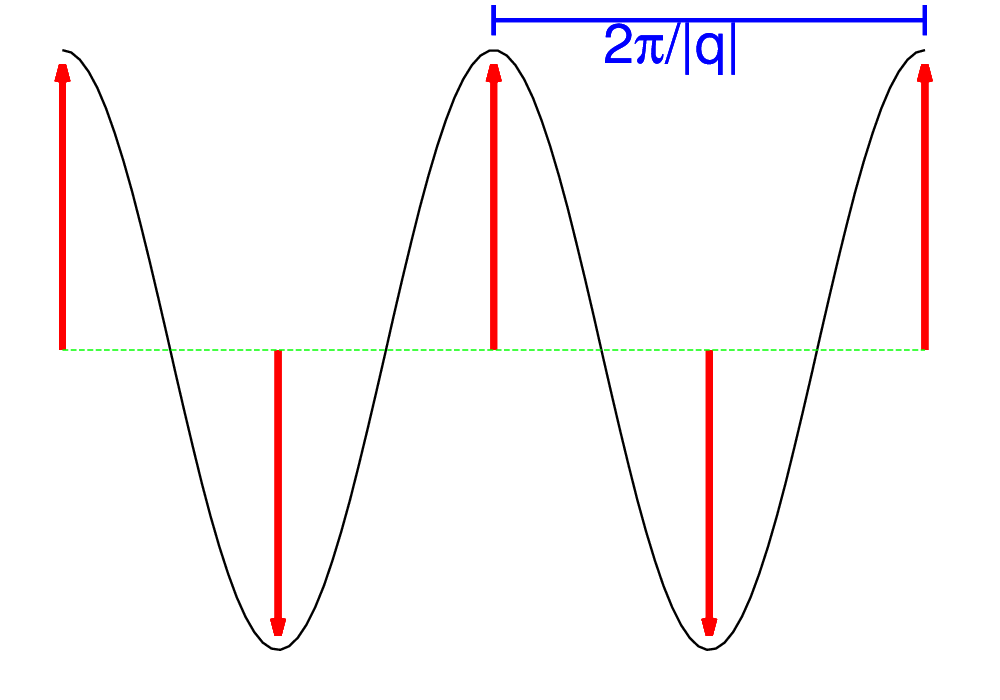
\includegraphics[scale=0.14]{./figures/q_diag.png}
\end{column}
\begin{column}{0.6\textwidth}
\centering
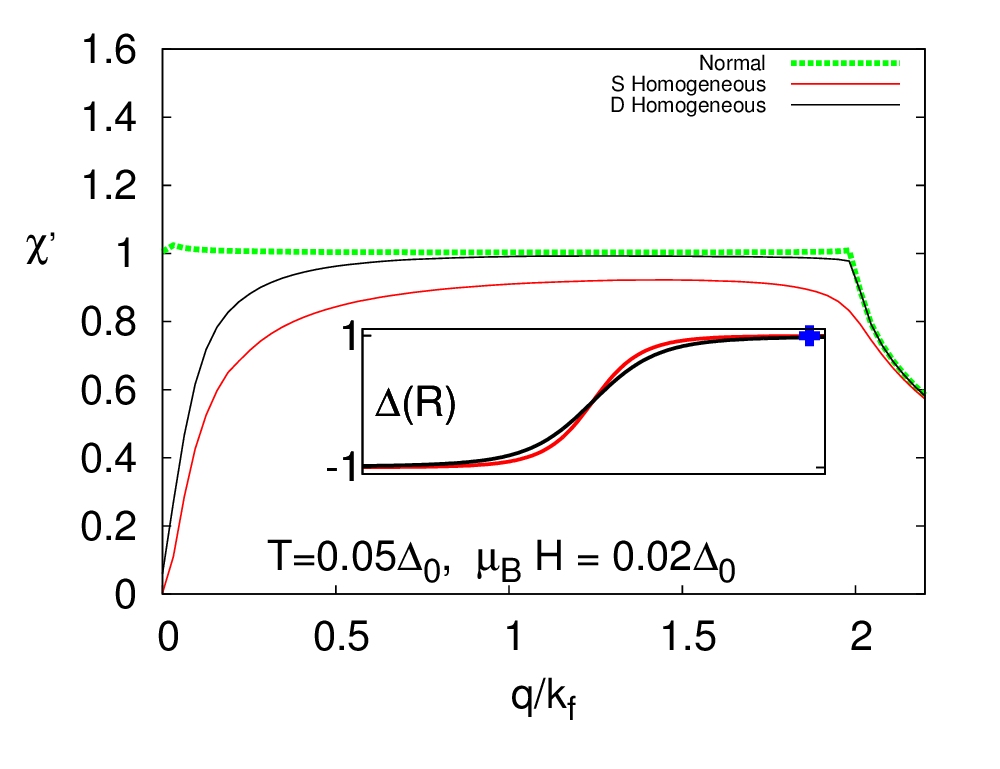
\includegraphics[scale=0.22]{./figures_3/fig_4/Fig4_1.png}\\
$\frac{\Delta_0}{\epsilon_f} = 0.05$,\quad static limit $\omega \rightarrow 0$
\end{column}
\end{columns}
\end{frame}
%%%%%%%%%%%%%%%%%%%%%%%%%%%%%%%%%%%%%%%%%%%%%%%%%%%%%%%%%%%%%%%%%%%%%%%%%%%%%%%%%%%%%%%%%%%%%%%%%%%%
\begin{frame} \frametitle{SUSCEPTIBILITY} 
PERTURBATION $\Rightarrow\,\,$ \fbox{$\cV = \mu_B\int d\vx \quad\Psi_\mu^\dagger(\vx,t) \vsigma_{\mu\nu}\cdot \delta \vH(\vx,t) \Psi_\nu(\vx,t)$} \\
$\chi_{_{\alpha\beta}}(\vx,\vx',\omega) = \frac{i\mu_B^2}{\chi_0}\int dt \quad e^{i\omega t}\langle [S_\alpha(\vx,t), S_\beta(\vx',0)]\theta(t) \rangle$
\begin{columns}
\begin{column}{0.42\textwidth}
$S_\alpha(\vx,t) = \Psi^\dagger_\mu(\vx,t) \sigma^{\alpha}_{\mu\nu}  \Psi^\dagger_\nu(\vx,t)$

\blue{\Fontvi $\Rightarrow$Transverse response \\\hspace{1cm}$(\alpha,\beta) = (x,x)\, or\, (y,y)$} \\

{\fbox{\red{$\chi(\vR,\vq) = \int d\vr e^{-i\vq\cdot\vr} \chi(\vR,\vr)$}}}

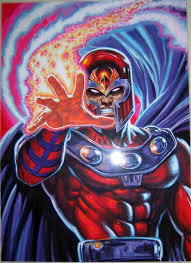
\includegraphics[scale=0.373]{./figures/para_magneto.jpg}
\end{column}
\begin{column}{0.6\textwidth}
\centering
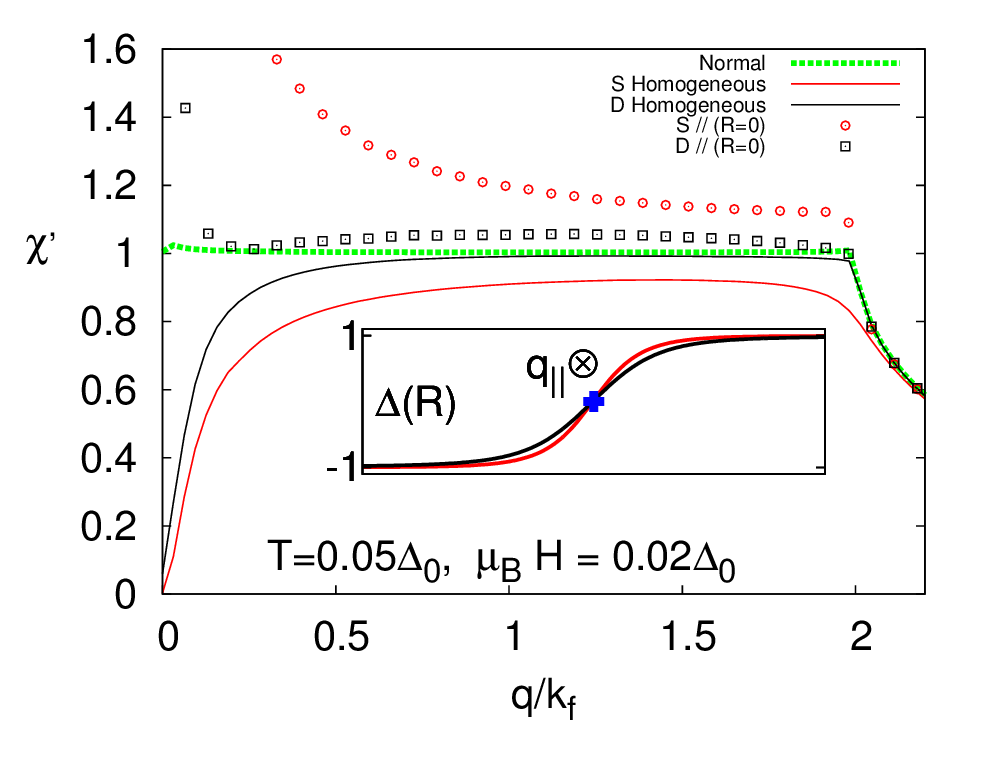
\includegraphics[scale=0.22]{./figures_3/fig_4/Fig4_2.png}\\
$\frac{\Delta_0}{\epsilon_f} = 0.05$,\quad static limit $\omega \rightarrow 0$
\end{column}
\end{columns}
\end{frame}
%%%%%%%%%%%%%%%%%%%%%%%%%%%%%%%%%%%%%%%%%%%%%%%%%%%%%%%%%%%%%%%%%%%%%%%%%%%%%%%%%%%%%%%%%%%%%%%
\begin{frame} \frametitle{SUSCEPTIBILITY} 
PERTURBATION $\Rightarrow\,\,$ \fbox{$\cV = \mu_B\int d\vx \quad\Psi_\mu^\dagger(\vx,t) \vsigma_{\mu\nu}\cdot \delta \vH(\vx,t) \Psi_\nu(\vx,t)$} \\
$\chi_{_{\alpha\beta}}(\vx,\vx',\omega) = \frac{i\mu_B^2}{\chi_0}\int dt \quad e^{i\omega t}\langle [S_\alpha(\vx,t), S_\beta(\vx',0)]\theta(t) \rangle$ 
\begin{columns}
\begin{column}{0.42\textwidth}
$S_\alpha(\vx,t) = \Psi^\dagger_\mu(\vx,t) \sigma^{\alpha}_{\mu\nu}  \Psi^\dagger_\nu(\vx,t)$

\blue{\Fontvi $\Rightarrow$Transverse response \\\hspace{1cm}$(\alpha,\beta) = (x,x)\, or\, (y,y)$} \\

{\fbox{\red{$\chi(\vR,\vq) = \int d\vr e^{-i\vq\cdot\vr} \chi(\vR,\vr)$}}}

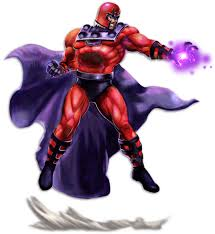
\includegraphics[scale=0.419]{./figures/perp_magneto.jpg}
\end{column}
\begin{column}{0.6\textwidth}
\centering
$\frac{\Delta_0}{\epsilon_f} = 0.05$,\quad static limit $\omega \rightarrow 0$
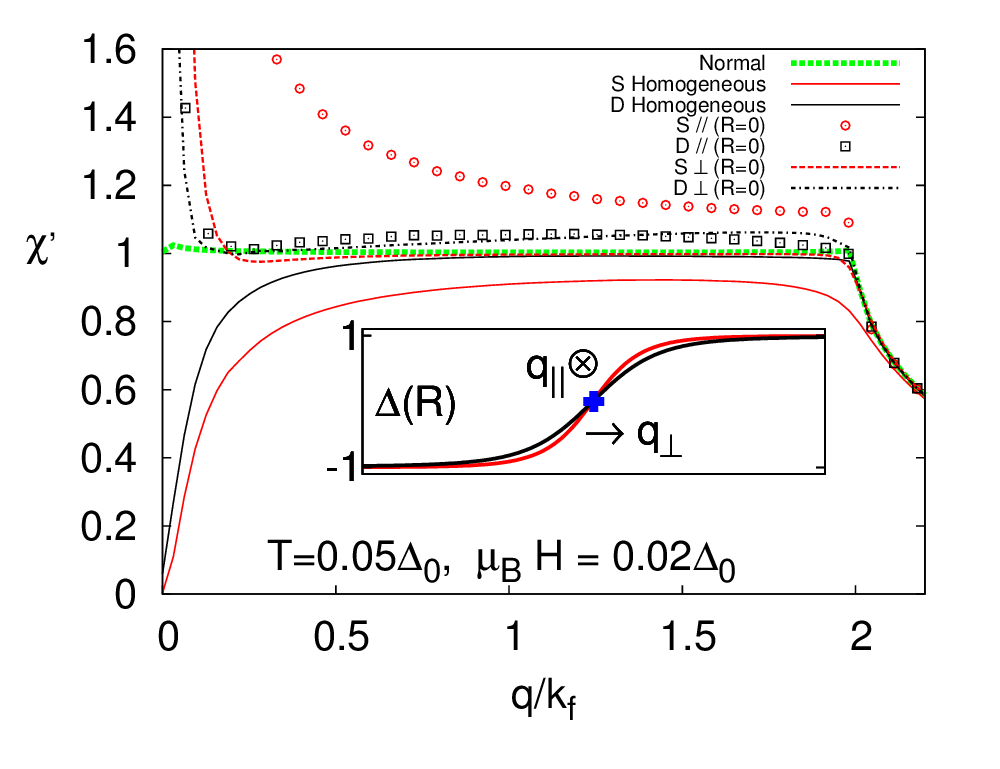
\includegraphics[scale=0.22]{./figures_3/fig_4/Fig4_3.png}\\
$\frac{\Delta_0}{\epsilon_f} = 0.05$,\quad static limit $\omega \rightarrow 0$
\end{column}
\end{columns}
\end{frame}
%%%%%%%%%%%%%%%%%%%%%%%%%%%%%%%%%%%%%%%%%%%%%%%%%%%%%%%%%%%%%%%%%%%%%%%%%%%%%%%%%%%%%%%%%%%%%%%
\begin{frame} \frametitle{SUSCEPTIBILITY} 
$\chi_{_i}(\vR,\vq)=\sum\limits_{\vn\vn'} {}^{i}\, X^{i}_{\vn\vn'}(\vR,\vq)$,\quad $i=\{I,\,\, II,\,\, III\}$
\begin{columns}
\begin{column}{0.4\textwidth}
	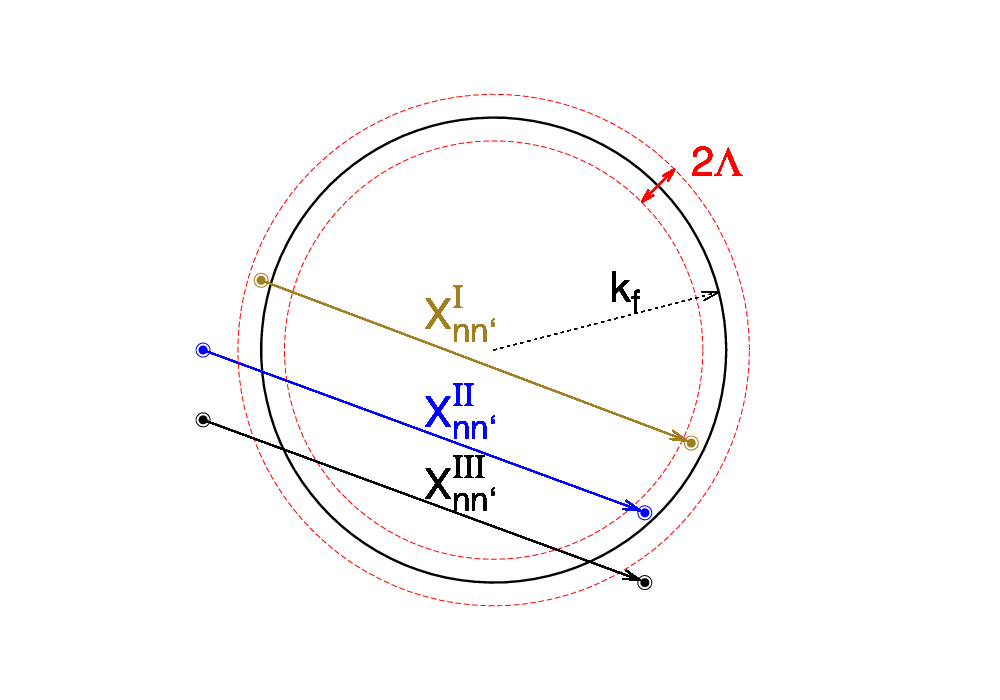
\includegraphics[scale=0.18]{./figures/sus_connection.png}\\
    \olive{$I$: $\epsilon_{\vn}< \Lambda,\,\,\epsilon_{\vn'} < \Lambda$} \\
	\blue{$II$: $\epsilon_{\vn}< \Lambda,\,\,\epsilon_{\vn'} > \Lambda$\\\hspace{1cm} $\vn \leftrightarrow \vn'$} \\
	\black{$III$: $\epsilon_{\vn}> \Lambda,\,\,\epsilon_{\vn'} > \Lambda$}
\end{column}
\begin{column}{0.6\textwidth}
\end{column}
\end{columns}
\end{frame}
%%%%%%%%%%%%%%%%%%%%%%%%%%%%%%%%%%%%%%%%%%%%%%%%%%%%%%%%%%%%%%%%%%%%%%%%%%%%%%%%%%%%%%%%%%%%%%%
\begin{frame} \frametitle{SUSCEPTIBILITY} 
$\chi_{_i}(\vR,\vq)=\sum\limits_{\vn\vn'} {}^{i}\, X^{i}_{\vn\vn'}(\vR,\vq)$,\quad $i=\{I,\,\, II,\,\, III\}$
\begin{columns}
\begin{column}{0.4\textwidth}
	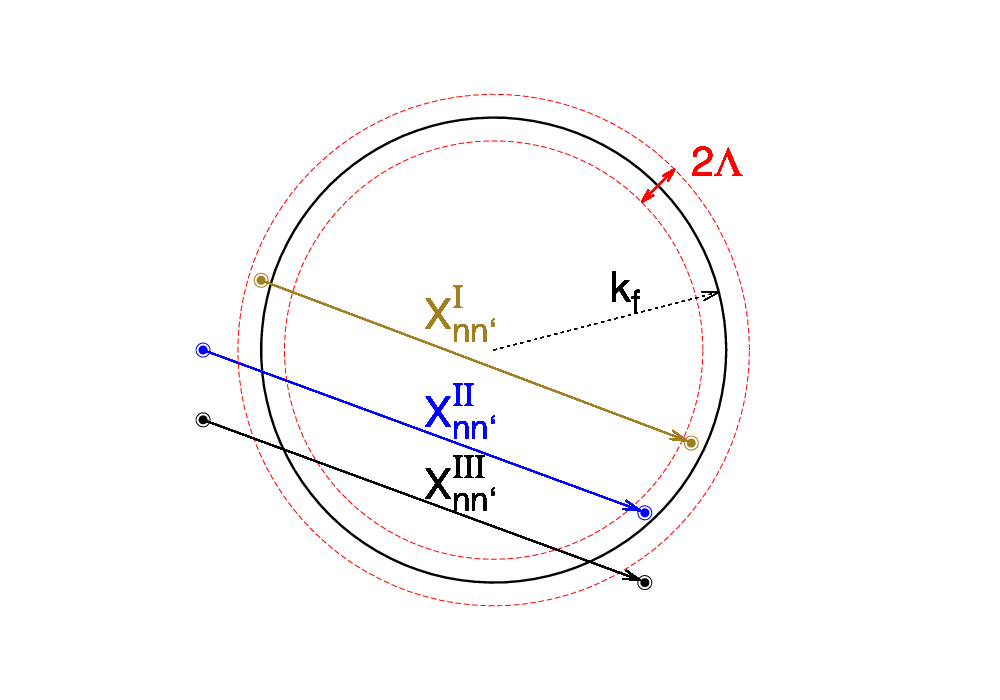
\includegraphics[scale=0.18]{./figures/sus_connection.png}\\
	\olive{$I$: $\epsilon_{\vn}< \Lambda,\,\,\epsilon_{\vn'} < \Lambda$} \\
	\blue{$II$: $\epsilon_{\vn}< \Lambda,\,\,\epsilon_{\vn'} > \Lambda$\\\hspace{1cm} $\vn \leftrightarrow \vn'$} \\
	\black{$III$: $\epsilon_{\vn}> \Lambda,\,\,\epsilon_{\vn'} > \Lambda$}
	
\end{column}
\begin{column}{0.6\textwidth}
\centering
\black{\huge$\delta\chi_{_i} = \chi_{_i} - \chi_{_i}^{N}$}
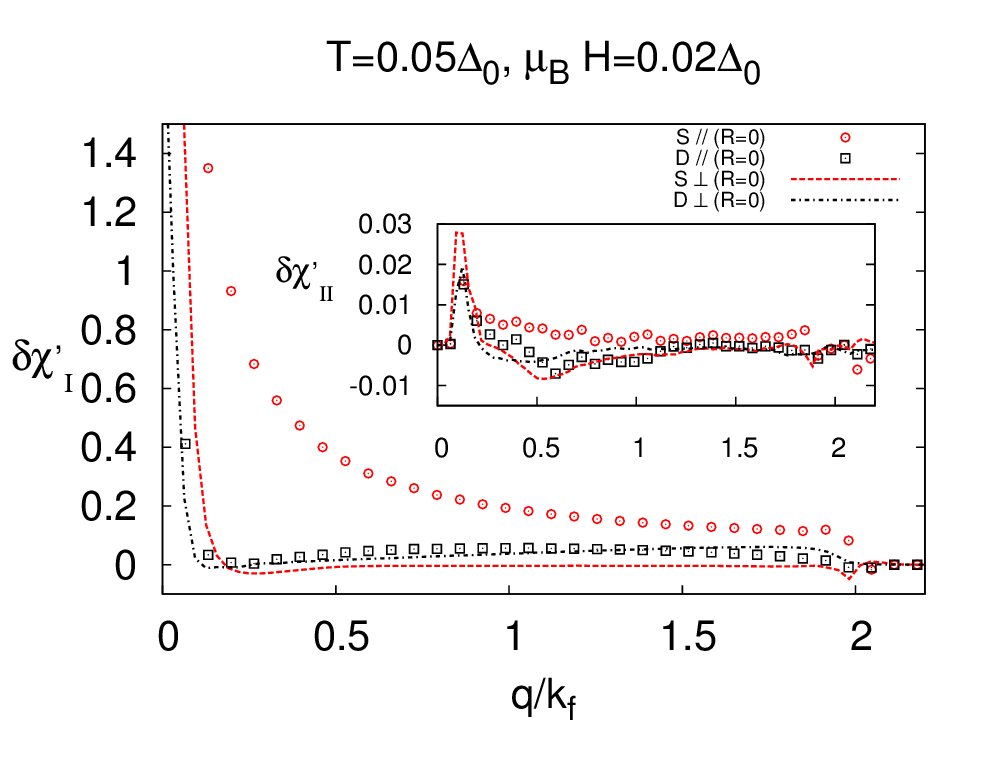
\includegraphics[scale=0.22]{./figures_3/fig_4/Fig4_delta.png}
\end{column}
\end{columns}
\end{frame}
%%%%%%%%%%%%%%%%%%%%%%%%%%%%%%%%%%%%%%%%%%%%%%%%%%%%%%%%%%%%%%%%%%%%%%%%%%%%%%%%%%%%%%%%%%%%%%%%%%%%%%%%%%%%%%%%%%%%%%%%%%%%
%%%%%%%%%%%%%%%%%%%%%%%%%%%%%%%%%%%%%%%%%%%%%%%%%%%%%%%%%%%%%%%%%%%%%%%%%%%%%%%%%%%%%%%%%%%%%%%%%%%%%%%%%%%%%%%%%%%%%%%%%%%%
%%%%%%%%%%%%%%%%%%%%%%%%%%%%%%%%%%%%%%%%%%%%%%%%%%%%%%%%%%%%%%%%%%%%%%%%%%%%%%%%%%%%%%%%%%%%%%%%%%%%%%%%%%%%%%%%%%%%%%%%%%%%
\begin{frame} \frametitle{ANDREEV APPROXIMATION} 
\hspace{5cm}\fbox{\huge $\vn\rightarrow (\hk,n)$} \\
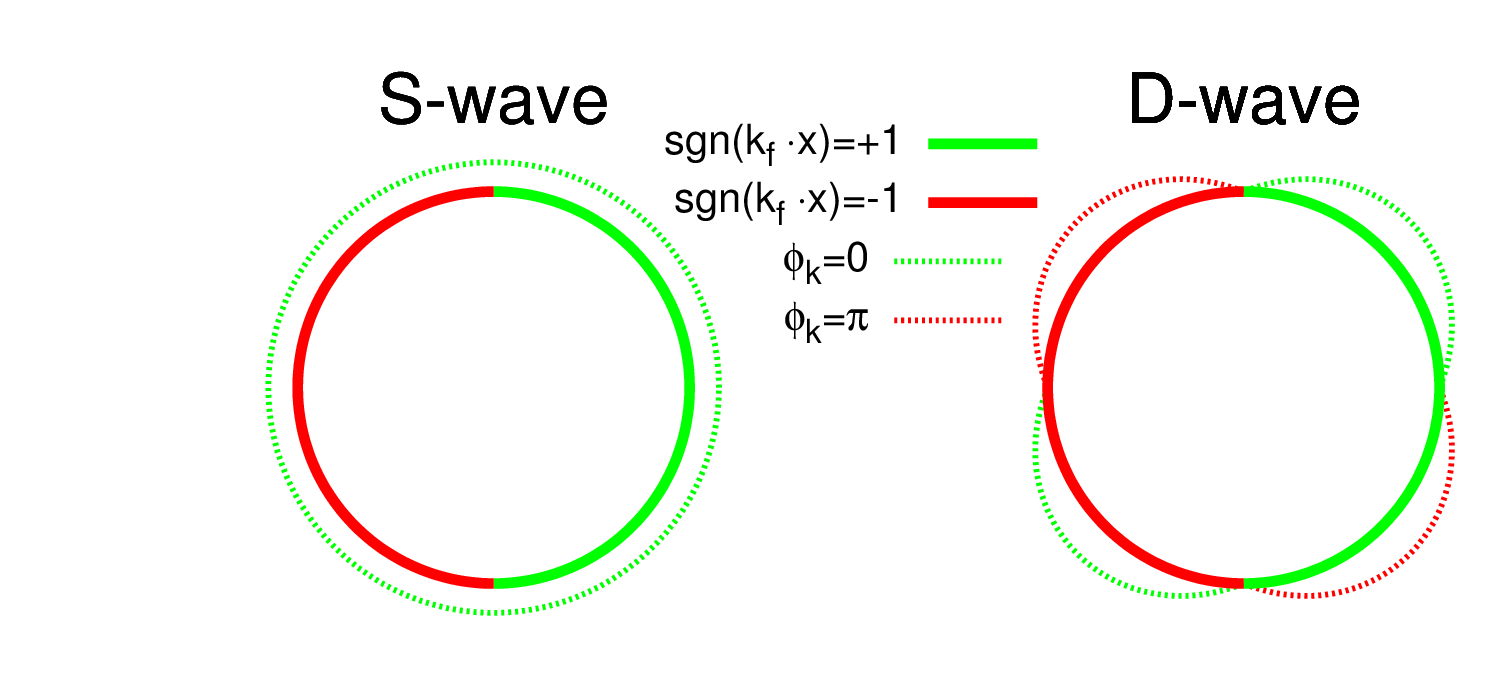
\includegraphics[scale=0.2]{./figures_3/fig2_SD_andreev/Fig2_1.png}\\ \vspace{0.39cm}
\fbox{LOWEST ENERGY STATE ALONG PARTICULAR $\hk$, $\rightarrow\epsilon_{\hk 0} << |\Delta_{\hk}|$} \\
\fbox{TRY TO MAXIMIZE SCATTERING AMPLITUDE $X^{I}_{\vn\vn'}(\vR,\vq)$}
\end{frame}
%%%%%%%%%%%%%%%%%%%%%%%%%%%%%%%%%%%%%%%%%%%%%%%%%%%%%%%%%%%%%%%%%%%%%%%%%%%%%%%%%%%%%%%%%%%%%%%
\begin{frame} \frametitle{ANDREEV APPROXIMATION} 
\hspace{5cm}\fbox{\huge $\vn\rightarrow (\hk,n)$} \\
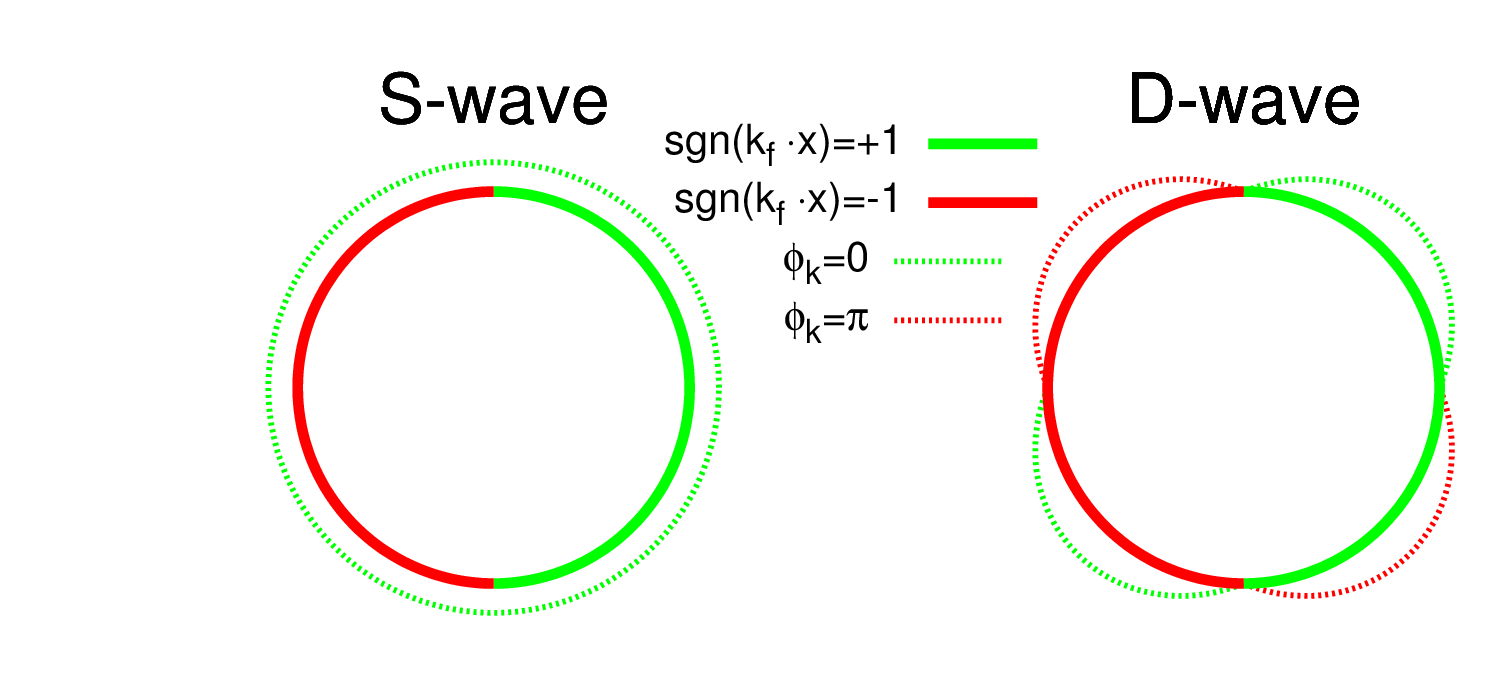
\includegraphics[scale=0.2]{./figures_3/fig2_SD_andreev/Fig2_1.png}\\
\fbox{\red{$\chi^{ABS}_{_I} =\sum\limits_{\hk\hk'\mu}$}\red{ $(1+S_{\hk\hk'})\Pi^+_{\hk\hk'\mu}$}\red{$+(1-S_{\hk\hk'})\Pi^-_{\hk\hk'\mu}$}} \hspace{0.45cm} \blue{\fbox{\Fontvi$\Pi^{\pm}_{\hk\hk'\mu} \propto \frac{1}{\epsilon_{\hk 0} \mp \epsilon_{\hk' 0} + 2\sigma^z_{\mu\mu}\mu_B H}$}}\\
\fbox{$S_{\hk\hk'}\approx e^{-i\zeta}$,\quad$\zeta = \frac{\pi}{2}(sgn(\hk\cdot\hx)-sgn(\Delta_{\hk})-sgn(\hk'\cdot\hx)+sgn(\Delta_{\hk'}))$}
\end{frame}
%%%%%%%%%%%%%%%%%%%%%%%%%%%%%%%%%%%%%%%%%%%%%%%%%%%%%%%%%%%%%%%%%%%%%%%%%%%%%%%%%%%%%%%%%%%%%%%
\begin{frame} \frametitle{ANDREEV APPROXIMATION} 
\hspace{5cm}\fbox{\huge $\vn\rightarrow (\hk,n)$} \\
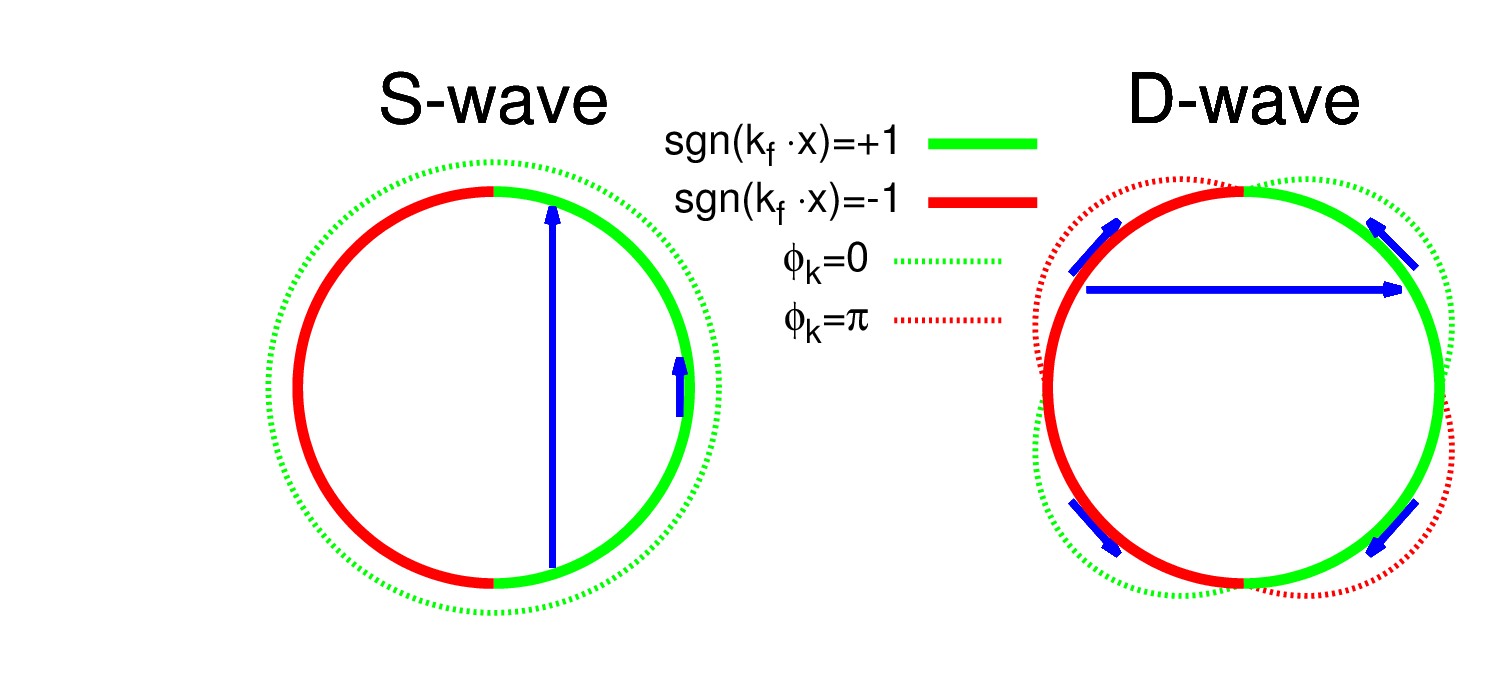
\includegraphics[scale=0.2]{./figures_3/fig2_SD_andreev/Fig2_2.png}\\
\fbox{\red{$\chi^{ABS}_{_I} =\sum\limits_{\hk\hk'\mu}$}\blue{ $(1+S_{\hk\hk'})\Pi^+_{\hk\hk'\mu}$}\red{$+(1-S_{\hk\hk'})\Pi^-_{\hk\hk'\mu}$}} \hspace{0.45cm} \blue{\fbox{$S_{\hk\hk'} = +1$, $\zeta = 0, \pm 4$}}\\
\fbox{$S_{\hk\hk'}\approx e^{-i\zeta}$,\quad$\zeta = \frac{\pi}{2}(sgn(\hk\cdot\hx)-sgn(\Delta_{\hk})-sgn(\hk'\cdot\hx)+sgn(\Delta_{\hk'}))$}
\end{frame}
%%%%%%%%%%%%%%%%%%%%%%%%%%%%%%%%%%%%%%%%%%%%%%%%%%%%%%%%%%%%%%%%%%%%%%%%%%%%%%%%%%%%%%%%%%%%%%%
\begin{frame} \frametitle{ANDREEV APPROXIMATION} 
\hspace{5cm}\fbox{\huge $\vn\rightarrow (\hk,n)$} \\
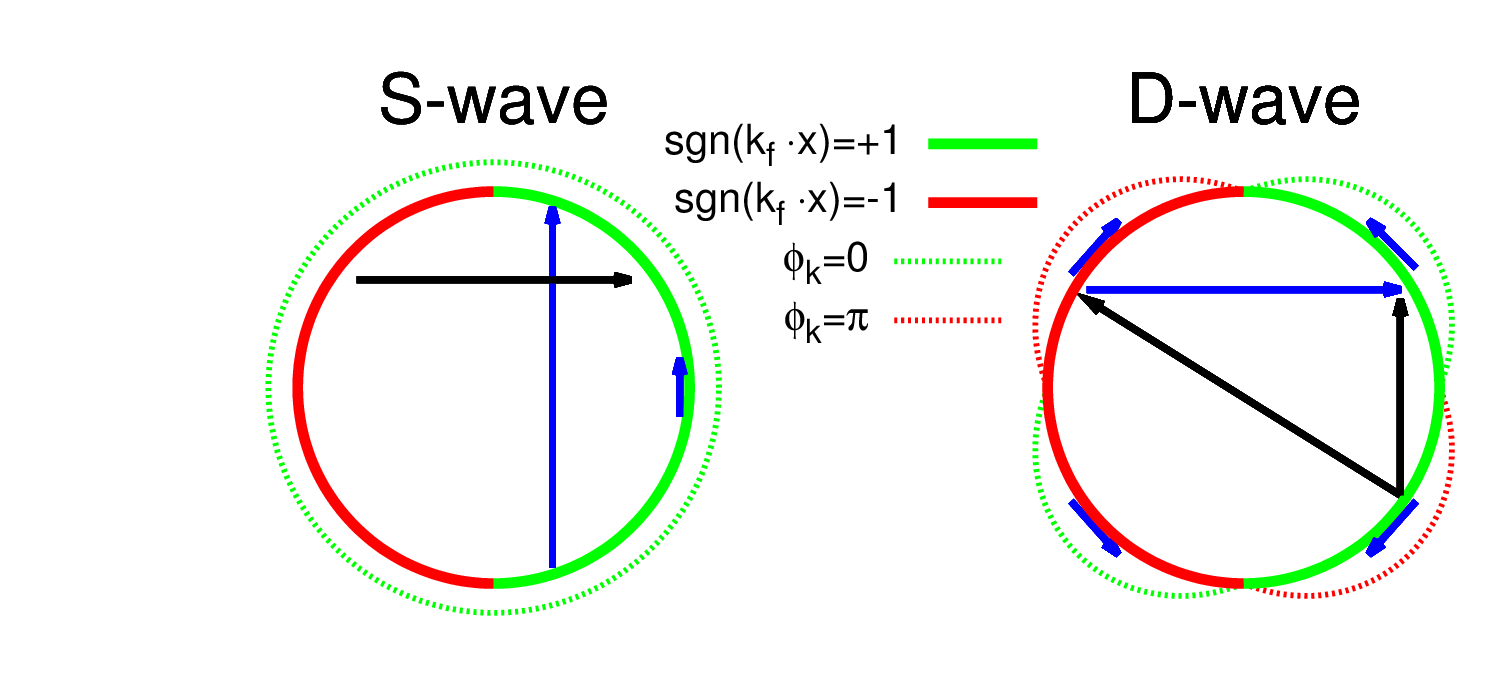
\includegraphics[scale=0.2]{./figures_3/fig2_SD_andreev/Fig2_3.png}\\
\fbox{\red{$\chi^{ABS}_{_I} =\sum\limits_{\hk\hk'\mu}$}\blue{ $(1+S_{\hk\hk'})\Pi^+_{\hk\hk'\mu}$}\black{$+(1-S_{\hk\hk'})\Pi^-_{\hk\hk'\mu}$}} \hspace{0.45cm} \black{\fbox{$S_{\hk\hk'} = -1$, $\zeta = \pm 2$}}\quad\\
\fbox{$S_{\hk\hk'}\approx e^{-i\zeta}$,\quad$\zeta = \frac{\pi}{2}(sgn(\hk\cdot\hx)-sgn(\Delta_{\hk})-sgn(\hk'\cdot\hx)+sgn(\Delta_{\hk'}))$}
\end{frame}
%%%%%%%%%%%%%%%%%%%%%%%%%%%%%%%%%%%%%%%%%%%%%%%%%%%%%%%%%%%%%%%%%%%%%%%%%%%%%%%%%%%%%%%%%%%%%%%%%%%%%%%%%%%%%%%%%%%%%%%%%%%%
%%%%%%%%%%%%%%%%%%%%%%%%%%%%%%%%%%%%%%%%%%%%%%%%%%%%%%%%%%%%%%%%%%%%%%%%%%%%%%%%%%%%%%%%%%%%%%%%%%%%%%%%%%%%%%%%%%%%%%%%%%%%
%%%%%%%%%%%%%%%%%%%%%%%%%%%%%%%%%%%%%%%%%%%%%%%%%%%%%%%%%%%%%%%%%%%%%%%%%%%%%%%%%%%%%%%%%%%%%%%%%%%%%%%%%%%%%%%%%%%%%%%%%%%%
\begin{frame}
\frametitle{SUSCEPTIBILITY \small{(ANDREEV APPROXIMATION)}}
{\huge REAL PART} $T=0.05\Delta_0$, $\mu_B H = 0.02\Delta_0$, $R=0$
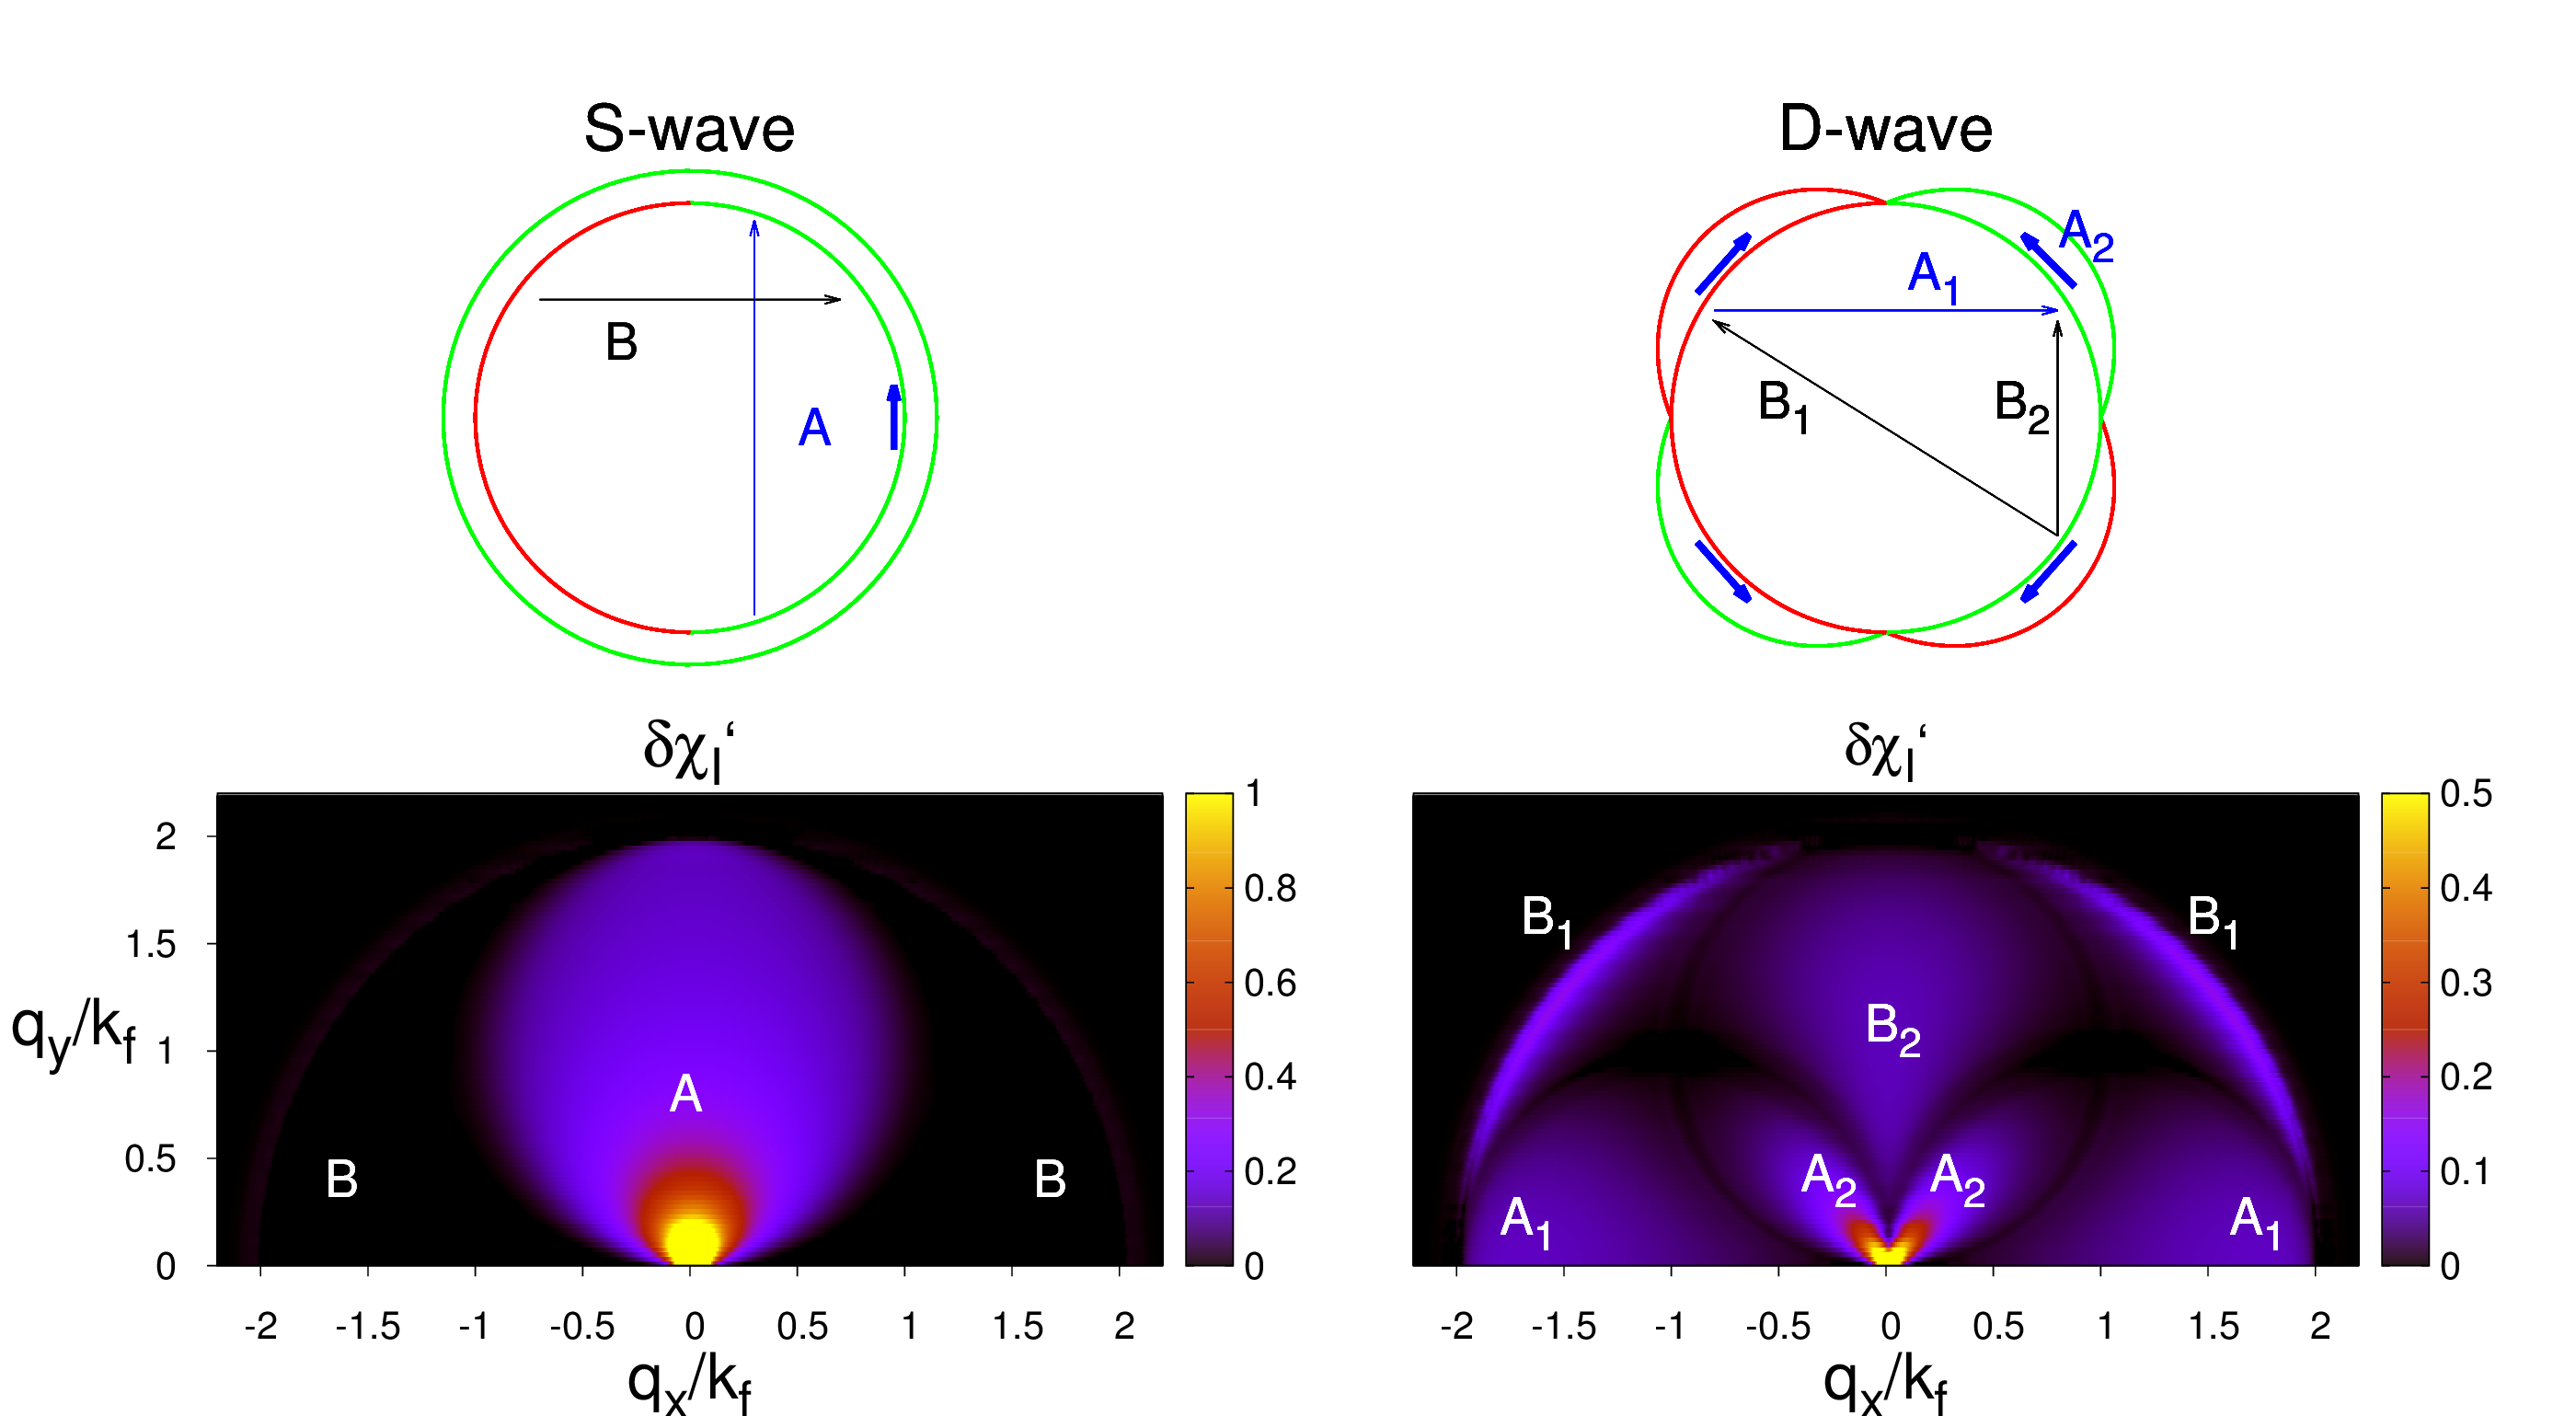
\includegraphics[scale=0.12]{./figures_3/fig2_SD_andreev/Fig2_andreev.png}

\end{frame}

%%%%%%%%%%%%%%%%%%%%%%%%%%%%%%%%%%%%%%%%%%%%%%%%%%%%%%%%%%%%%%%%%%%%%%%%%%%%%%%%%%%%%%%%%%%%%%%%%%%%%%%%%%%%%%%%%%%%%%%%%%%%
%%%%%%%%%%%%%%%%%%%%%%%%%%%%%%%%%%%%%%%%%%%%%%%%%%%%%%%%%%%%%%%%%%%%%%%%%%%%%%%%%%%%%%%%%%%%%%%%%%%%%%%%%%%%%%%%%%%%%%%%%%%%
%%%%%%%%%%%%%%%%%%%%%%%%%%%%%%%%%%%%%%%%%%%%%%%%%%%%%%%%%%%%%%%%%%%%%%%%%%%%%%%%%%%%%%%%%%%%%%%%%%%%%%%%%%%%%%%%%%%%%%%%%%%%
\begin{frame} \frametitle{FERROMAGNETIC RESPONSE}
\fbox{\huge $\rightarrow$ decreasing with temperature and field${}^*$} \\
\vspace{1cm}
\begin{columns}
\begin{column}{0.5\textwidth}
\centering S WAVE (R=0)
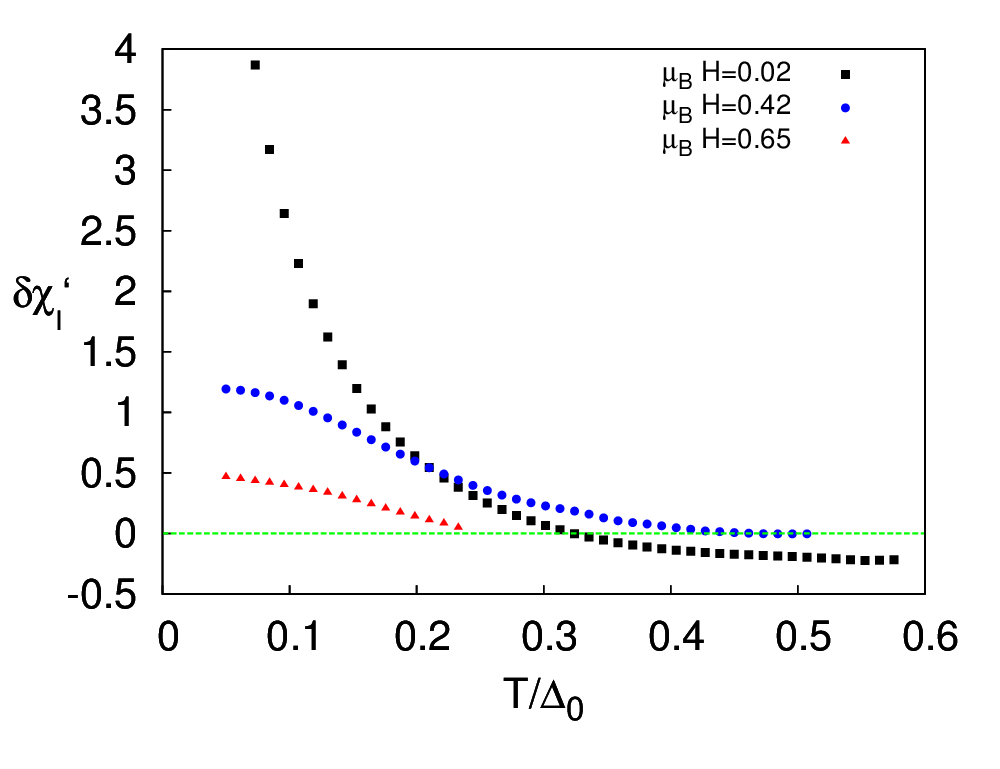
\includegraphics[scale=0.17]{./figures_3/fig_5/Fig5S_1.png} \\
\end{column}
\begin{column}{0.5\textwidth}
\centering D WAVE (R=0)
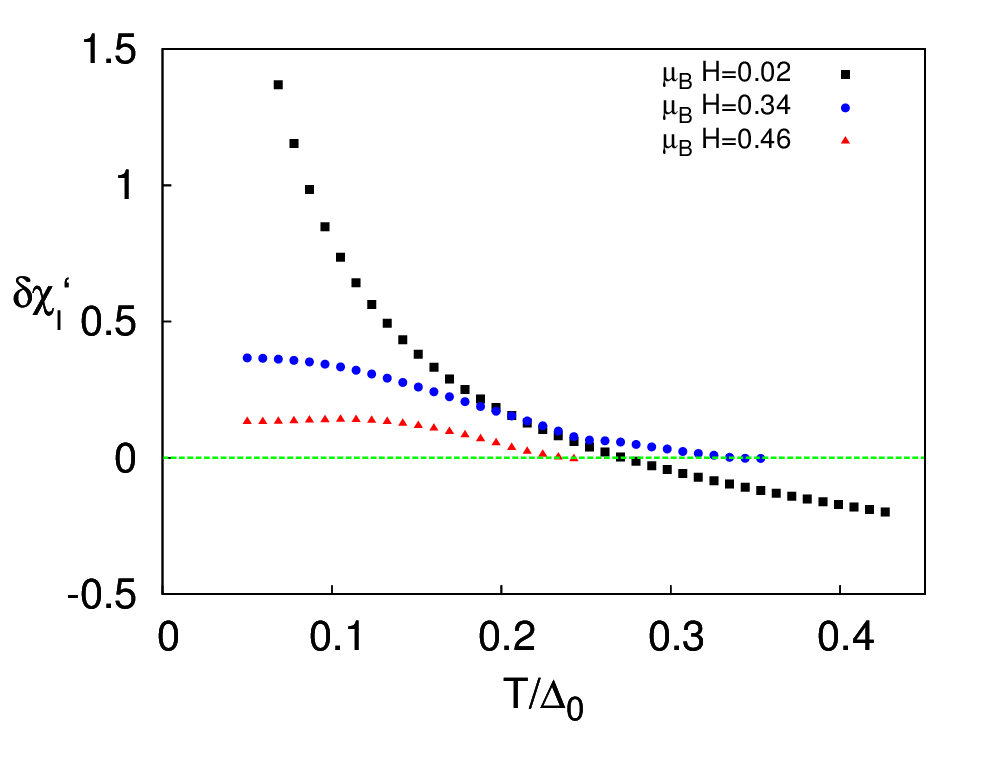
\includegraphics[scale=0.17]{./figures_3/fig_5/Fig5D_1.png} \\
\end{column}
\end{columns}
${}^*$ Excluding narrow region near $\mu_B H =0$ 
\end{frame}
%%%%%%%%%%%%%%%%%%%%%%%%%%%%%%%%%%%%%%%%%%%%%%%%%%%%%%%%%%%%%%%%%%%%%%%%%%%%%%%%%%%%%%%%%%%%%%%%%%%%%%%%%%%%%%%%%%%%%%%%%%%%
%%%%%%%%%%%%%%%%%%%%%%%%%%%%%%%%%%%%%%%%%%%%%%%%%%%%%%%%%%%%%%%%%%%%%%%%%%%%%%%%%%%%%%%%%%%%%%%%%%%%%%%%%%%%%%%%%%%%%%%%%%%%
%%%%%%%%%%%%%%%%%%%%%%%%%%%%%%%%%%%%%%%%%%%%%%%%%%%%%%%%%%%%%%%%%%%%%%%%%%%%%%%%%%%%%%%%%%%%%%%%%%%%%%%%%%%%%%%%%%%%%%%%%%%%
\begin{frame}
\frametitle{RELAXATION RATE}
{\huge IMAGINARY PART} $T=0.05\Delta_0$, $\mu_B H = 0.02\Delta_0$, $R=0$
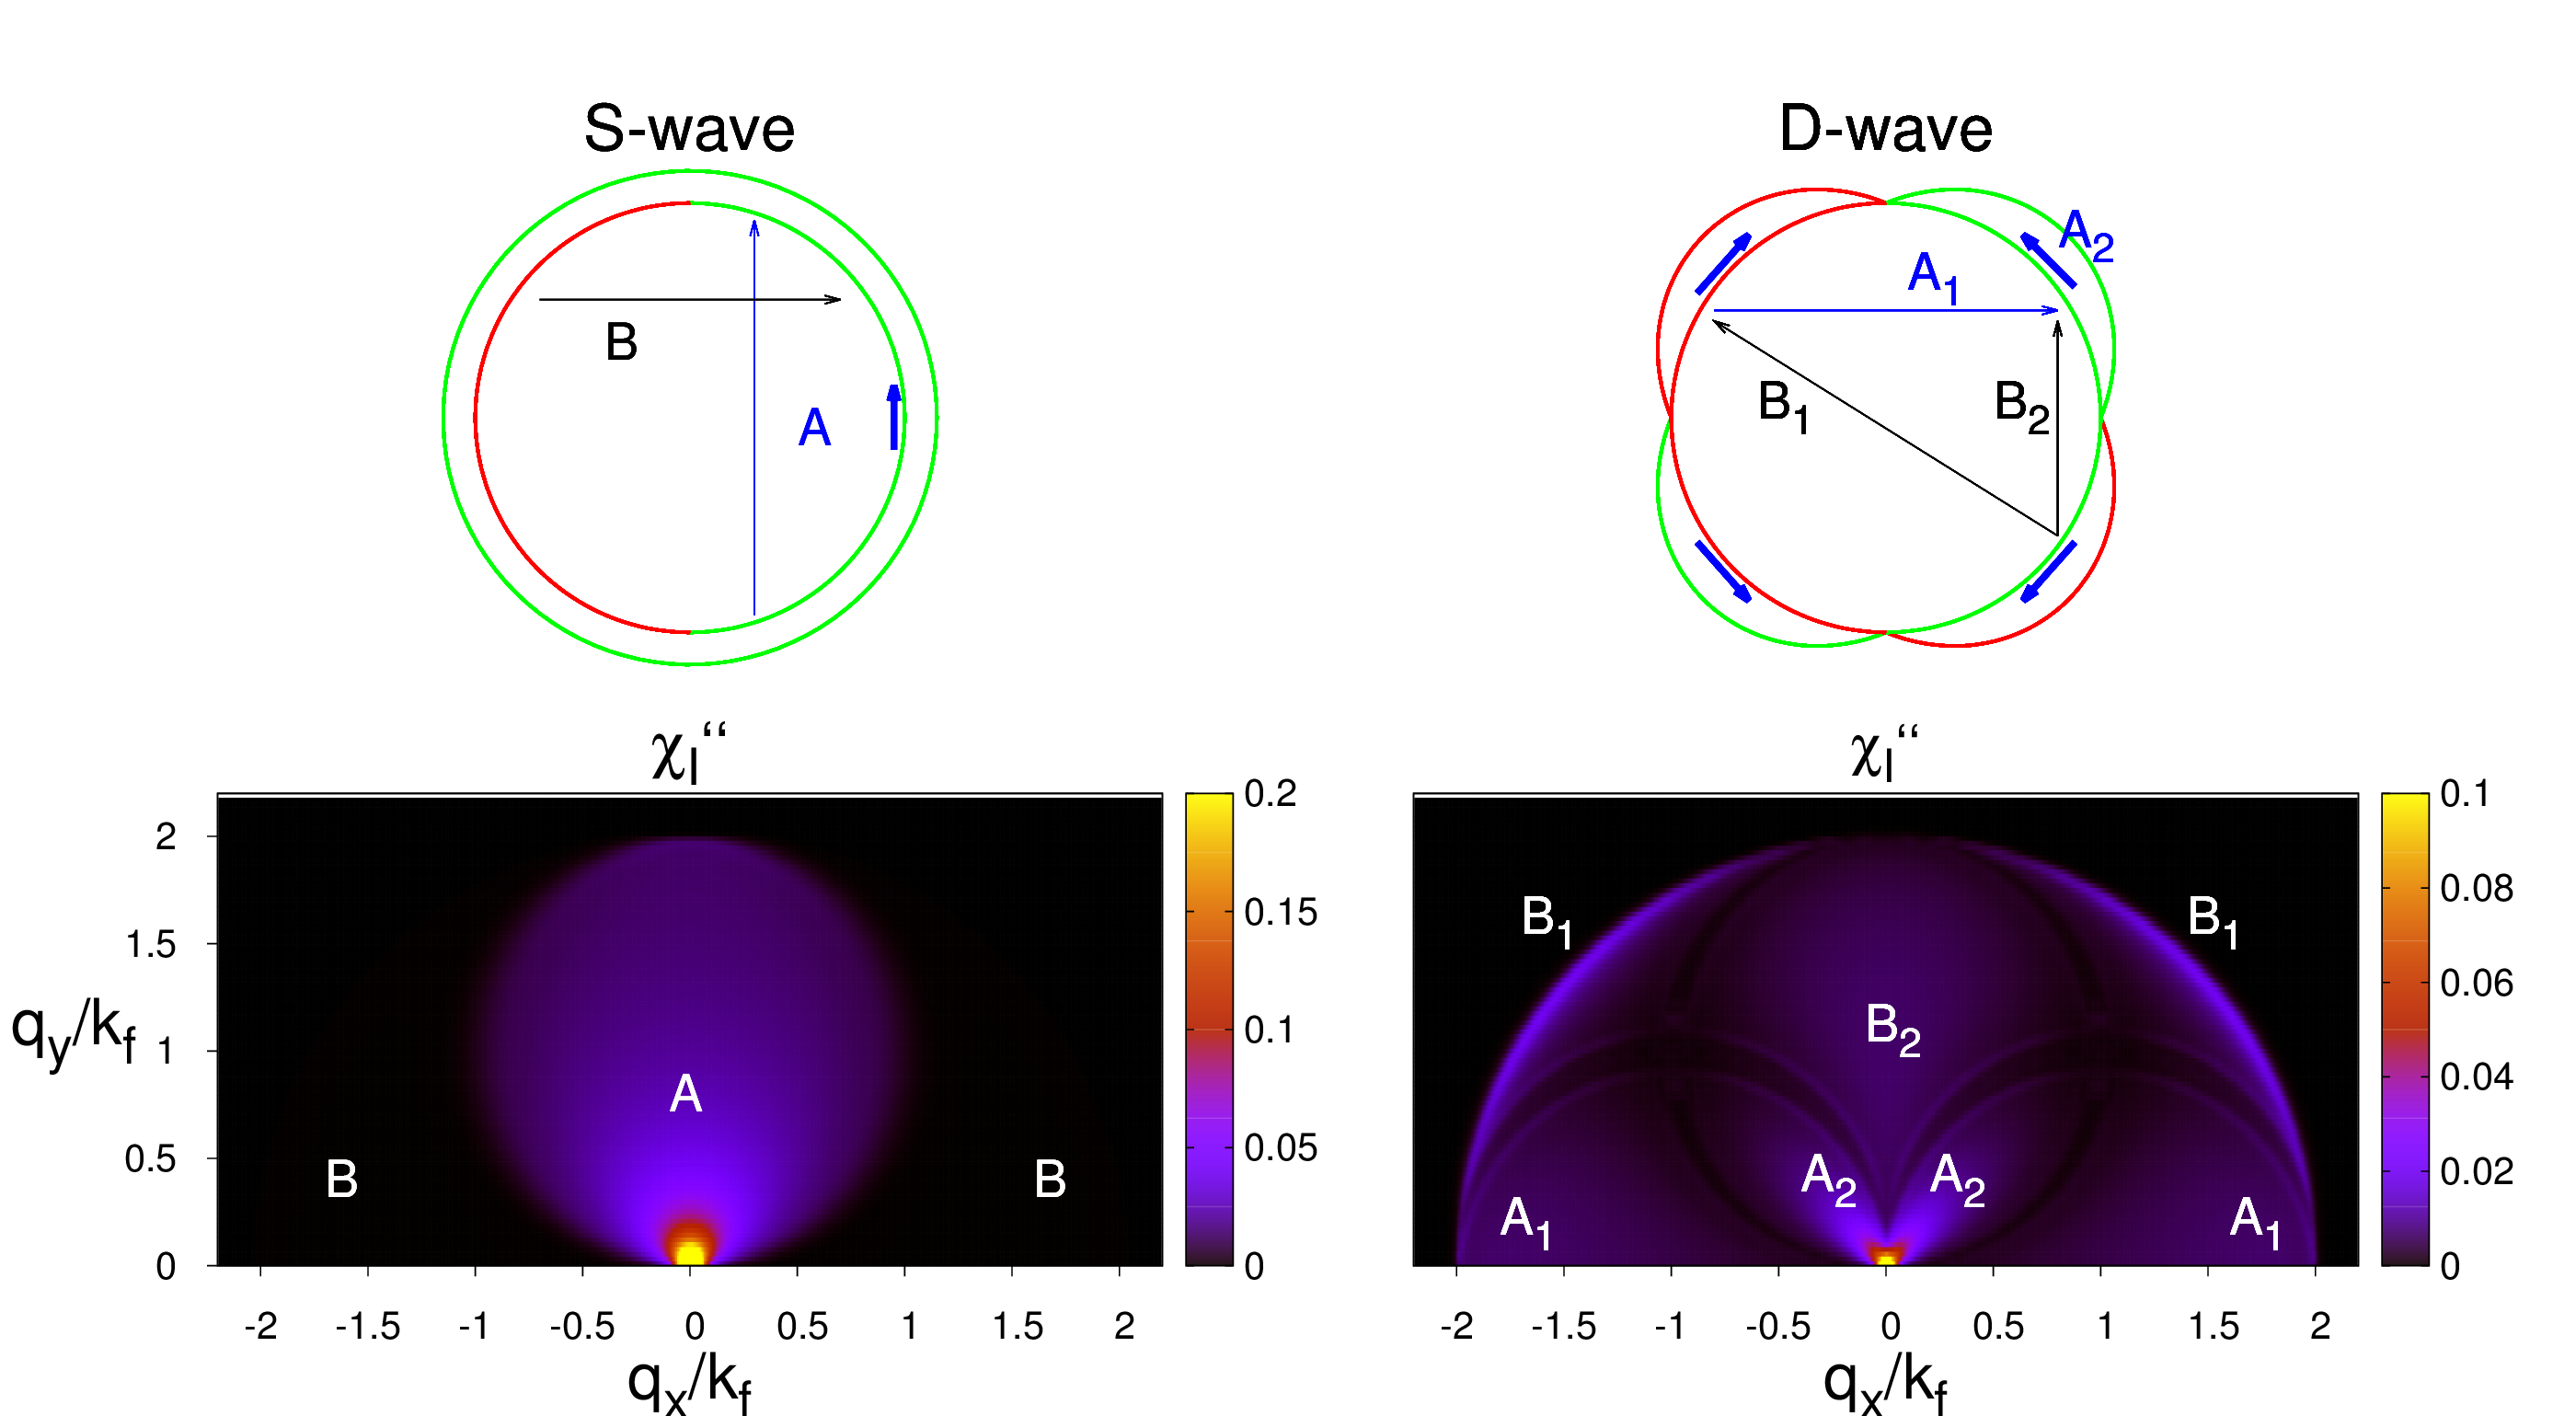
\includegraphics[scale=0.12]{./figures_3/fig2_SD_andreev/Fig2_andreev_imag.png}

\end{frame}
%%%%%%%%%%%%%%%%%%%%%%%%%%%%%%%%%%%%%%%%%%%%%%%%%%%%%%%%%%%%%%%%%%%%%%%%%%%%%%%%%%%%%%%%%%%%%%%%%%%%%%%%%%%%%%%%%%%%%%%%%%%%
%%%%%%%%%%%%%%%%%%%%%%%%%%%%%%%%%%%%%%%%%%%%%%%%%%%%%%%%%%%%%%%%%%%%%%%%%%%%%%%%%%%%%%%%%%%%%%%%%%%%%%%%%%%%%%%%%%%%%%%%%%%%
%%%%%%%%%%%%%%%%%%%%%%%%%%%%%%%%%%%%%%%%%%%%%%%%%%%%%%%%%%%%%%%%%%%%%%%%%%%%%%%%%%%%%%%%%%%%%%%%%%%%%%%%%%%%%%%%%%%%%%%%%%%%
\begin{frame} \frametitle{RELAXATION RATE}
\centering \red{$(TT_1)^{-1}(\vR) =\frac{1}{\omega} \sum_{\vq} \cI m (\chi_{_{\perp I}}(\vR,\vq))$}\\
\fbox{\olive{Korringa (normal) limit\quad $\Rightarrow$\quad $(TT_1)^{-1} = constant$}}
\vspace{1cm}
\begin{columns}
\begin{column}{0.5\textwidth}
\centering S WAVE (R=0)
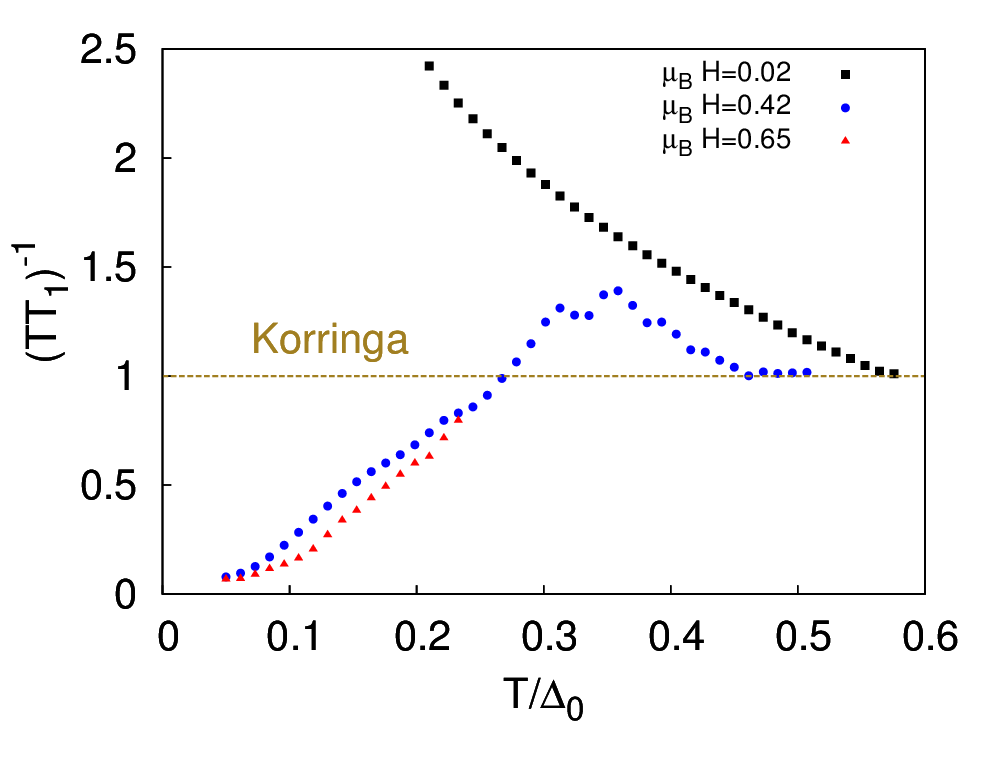
\includegraphics[scale=0.17]{./figures_3/fig_5/Fig5S_2.png} \\
\end{column}
\begin{column}{0.5\textwidth}
\centering D WAVE (R=0)
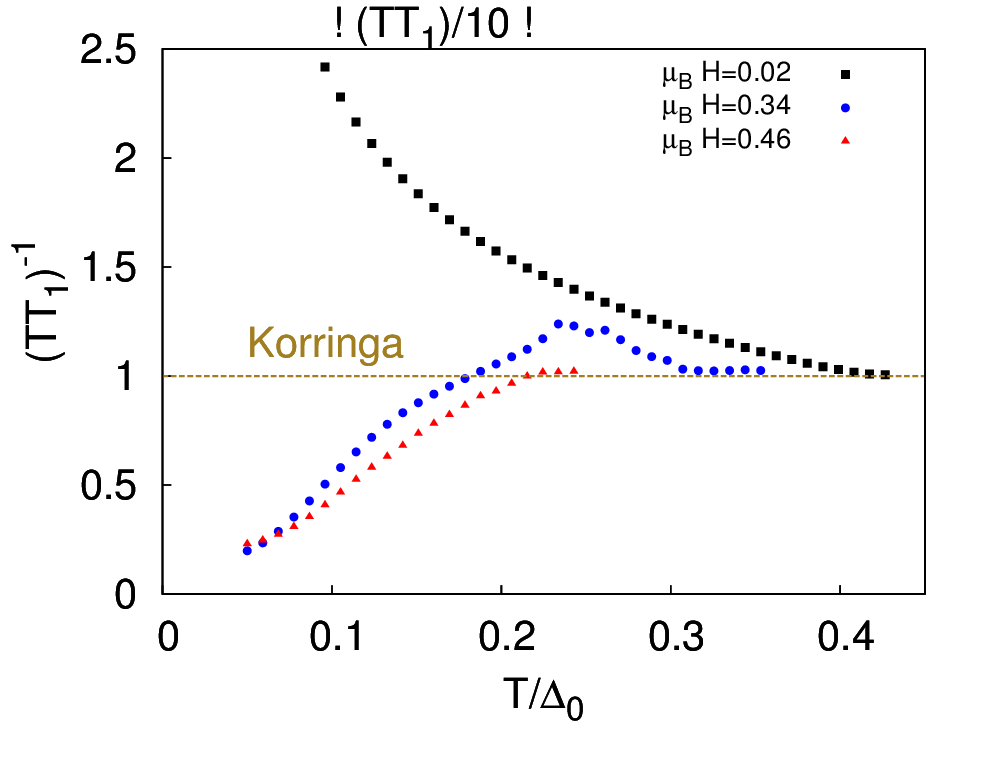
\includegraphics[scale=0.17]{./figures_3/fig_5/Fig5D_2.png} \\
\end{column}
\end{columns}

\end{frame}
%%%%%%%%%%%%%%%%%%%%%%%%%%%%%%%%%%%%%%%%%%%%%%%%%%%%%%%%%%%%%%%%%%%%%%%%%%%%%%%%%%%%%%%%%%%%%%%%%%%%%%%%%%%%%%%%%%%%%%%%%%%%
%%%%%%%%%%%%%%%%%%%%%%%%%%%%%%%%%%%%%%%%%%%%%%%%%%%%%%%%%%%%%%%%%%%%%%%%%%%%%%%%%%%%%%%%%%%%%%%%%%%%%%%%%%%%%%%%%%%%%%%%%%%%
%%%%%%%%%%%%%%%%%%%%%%%%%%%%%%%%%%%%%%%%%%%%%%%%%%%%%%%%%%%%%%%%%%%%%%%%%%%%%%%%%%%%%%%%%%%%%%%%%%%%%%%%%%%%%%%%%%%%%%%%%%%%
\begin{frame} \frametitle{RELAXATION RATE}

\begin{columns}
\begin{column}{0.5\textwidth}
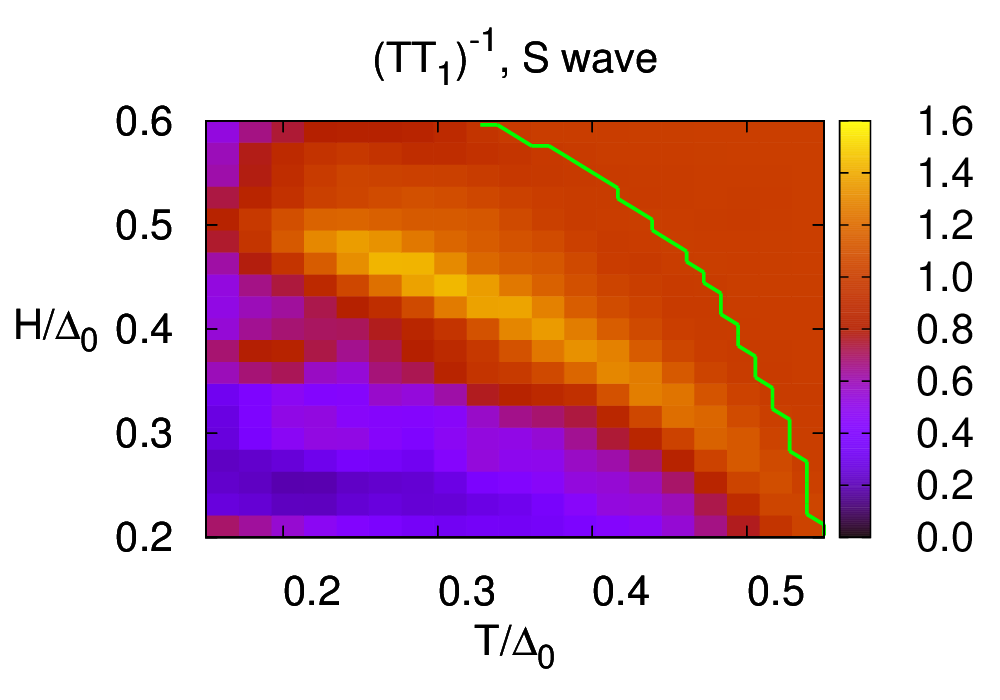
\includegraphics[scale=0.17]{./figures_3/fig3_S/Fig3.png}
\end{column}
\begin{column}{0.5\textwidth}
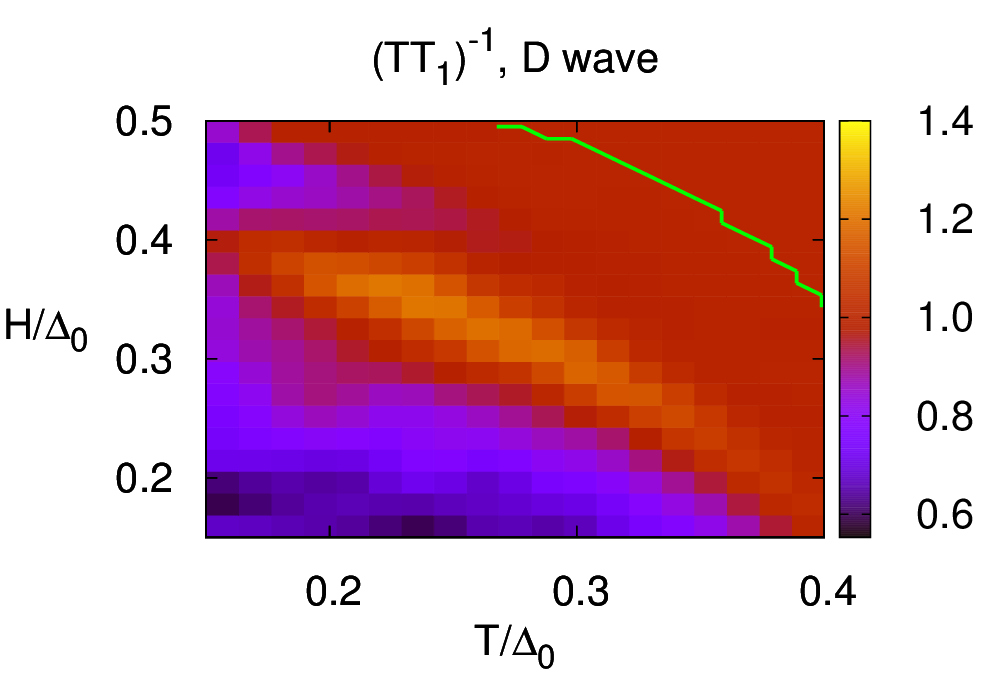
\includegraphics[scale=0.17]{./figures_3/fig3_D/Fig3.png}
\end{column}
\end{columns}
\begin{columns}
\begin{column}{0.4\textwidth}
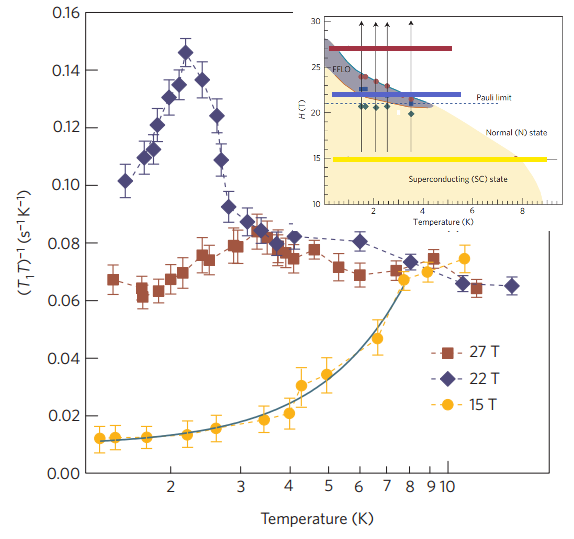
\includegraphics[scale=0.2]{./figures/organic_T1.png}
\end{column}
\begin{column}{0.7\textwidth}
?? Will this enhancement change in H-T if...\\
\quad a) we move DWs closer together? \\
\quad b) we allow $\Delta$ to change phase?
\end{column}
\end{columns}
\end{frame}

%%%%%%%%%%%%%%%%%%%%%%%%%%%%%%%%%%%%%%%%%%%%%%%%%%%%%%%%%%%%%%%%%%%%%%%%%%%%%%%%%%%%%%%%%%%%%%%%%%%%%%%%%%%%%%%%%%%%%%%%%%%%
%%%%%%%%%%%%%%%%%%%%%%%%%%%%%%%%%%%%%%%%%%%%%%%%%%%%%%%%%%%%%%%%%%%%%%%%%%%%%%%%%%%%%%%%%%%%%%%%%%%%%%%%%%%%%%%%%%%%%%%%%%%%
%%%%%%%%%%%%%%%%%%%%%%%%%%%%%%%%%%%%%%%%%%%%%%%%%%%%%%%%%%%%%%%%%%%%%%%%%%%%%%%%%%%%%%%%%%%%%%%%%%%%%%%%%%%%%%%%%%%%%%%%%%%%
\begin{frame}\frametitle{Conclusions}
Conditions for magnetic coherence of bound states near a domain wall \\
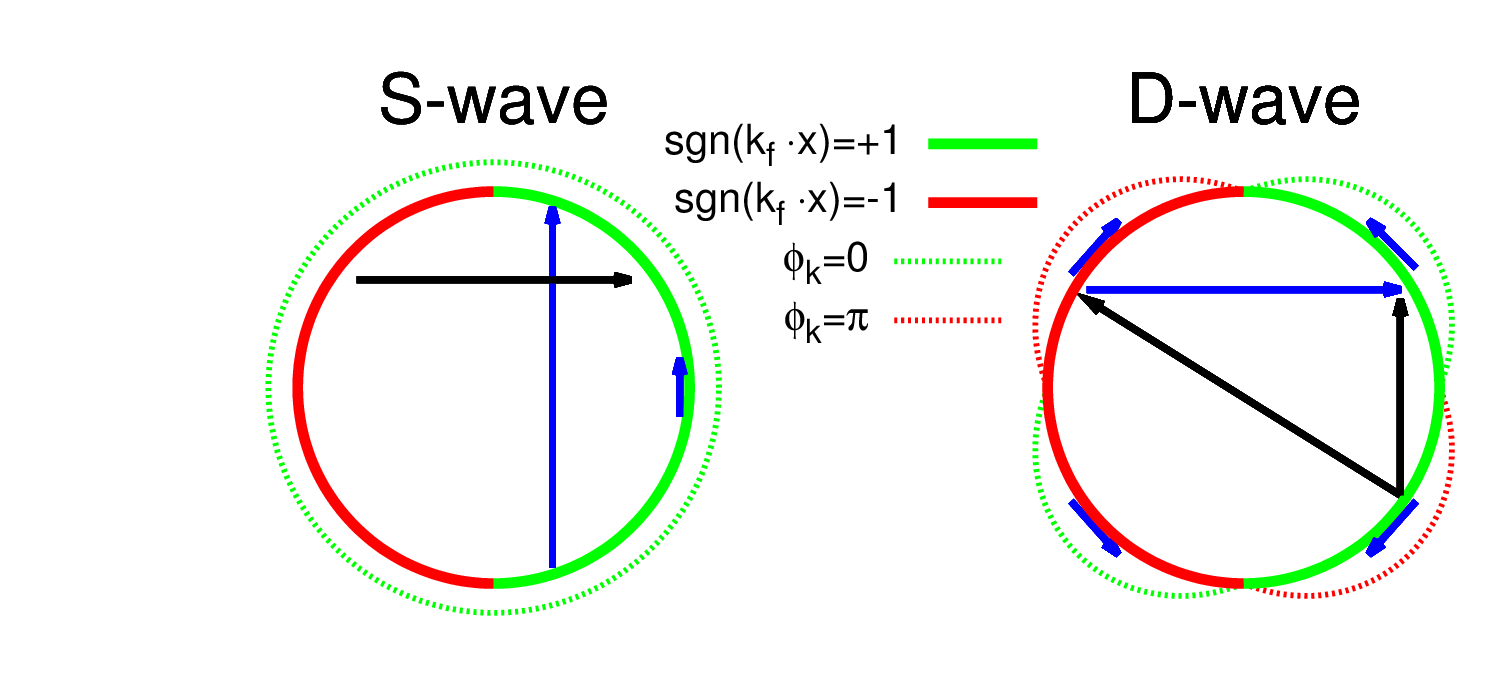
\includegraphics[scale=0.1]{./figures_3/fig2_SD_andreev/Fig2_3.png}
% \fbox{Increases $\chi_{\perp}(\vq)$} 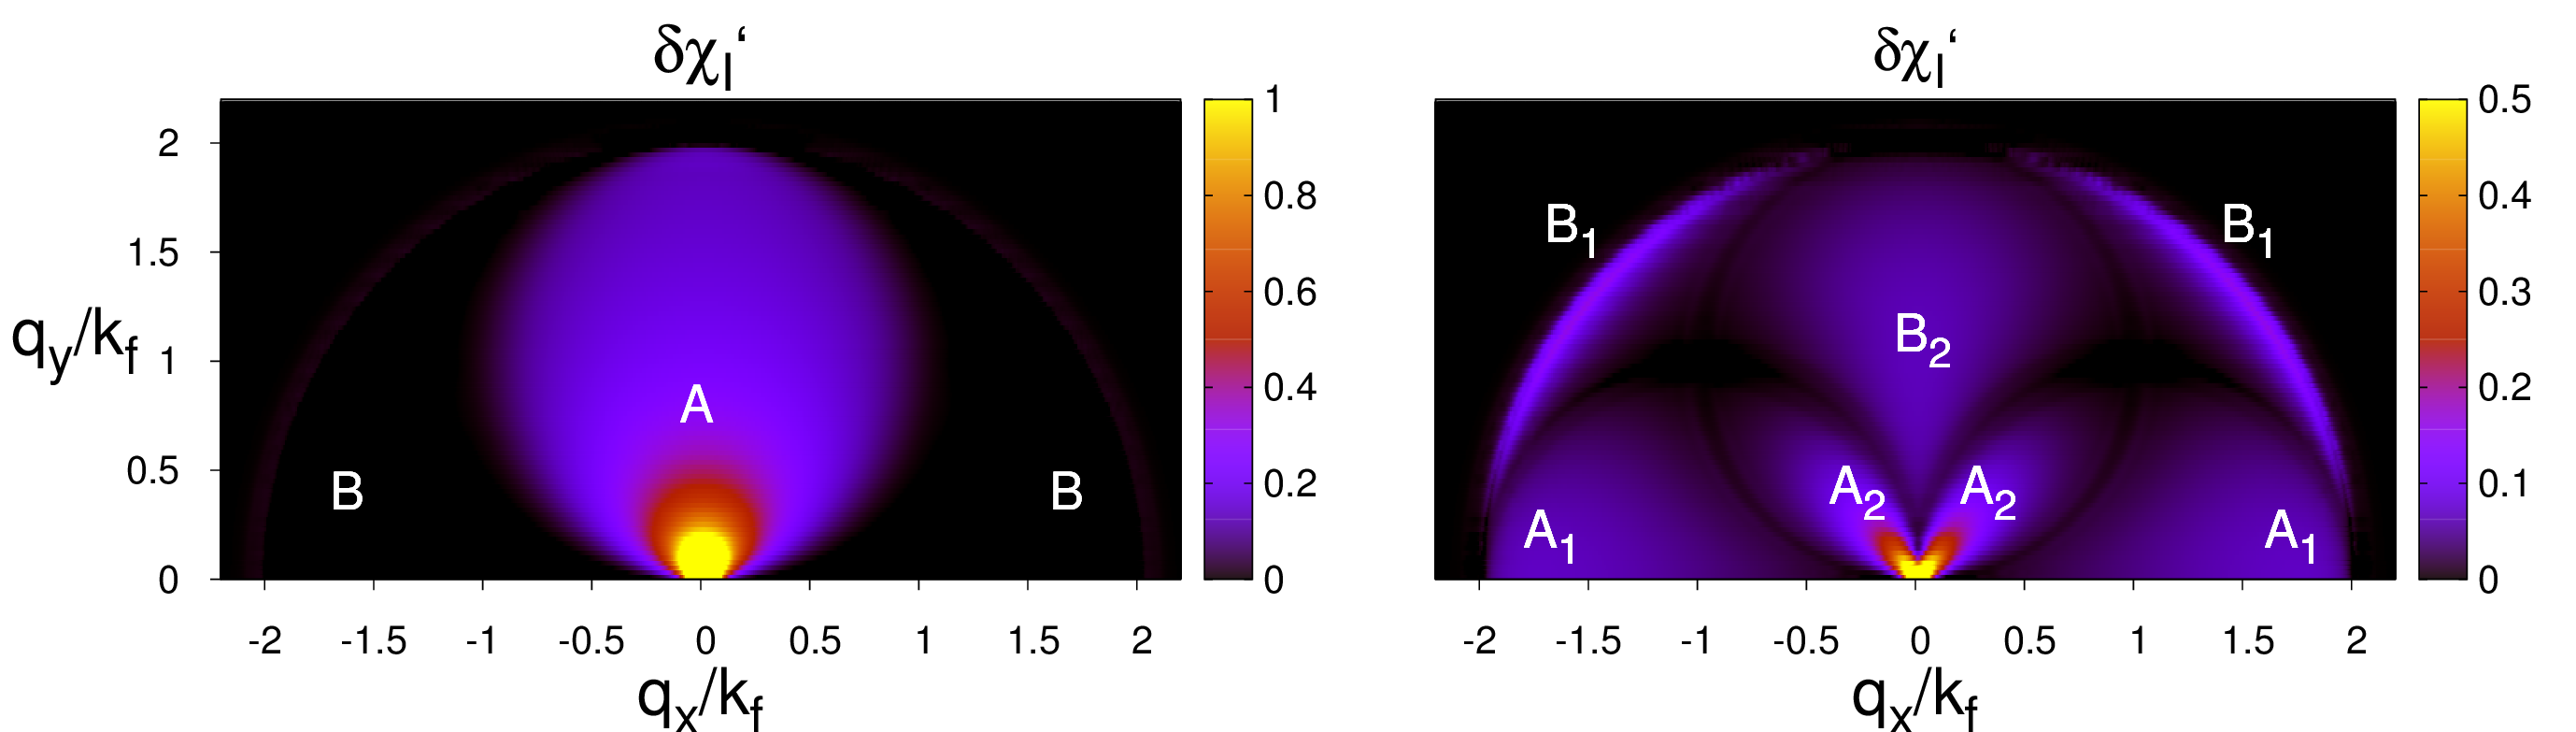
\includegraphics[scale=0.07]{./figures_3/fig2_SD_andreev/Fig2_andreev_cut.png}\\
%\fbox{Increases $(TT_1)_{\perp}^{-1}$} 
\begin{columns}
\begin{column}{0.35\textwidth}
 \fbox{Increases $\chi_{_\perp}(\vq)$} $\Rightarrow$ \\
 \vspace{2cm}
\fbox{Increases $(TT_1)_{\perp}^{-1}$} $\Rightarrow$
\end{column}
\begin{column}{0.7\textwidth}
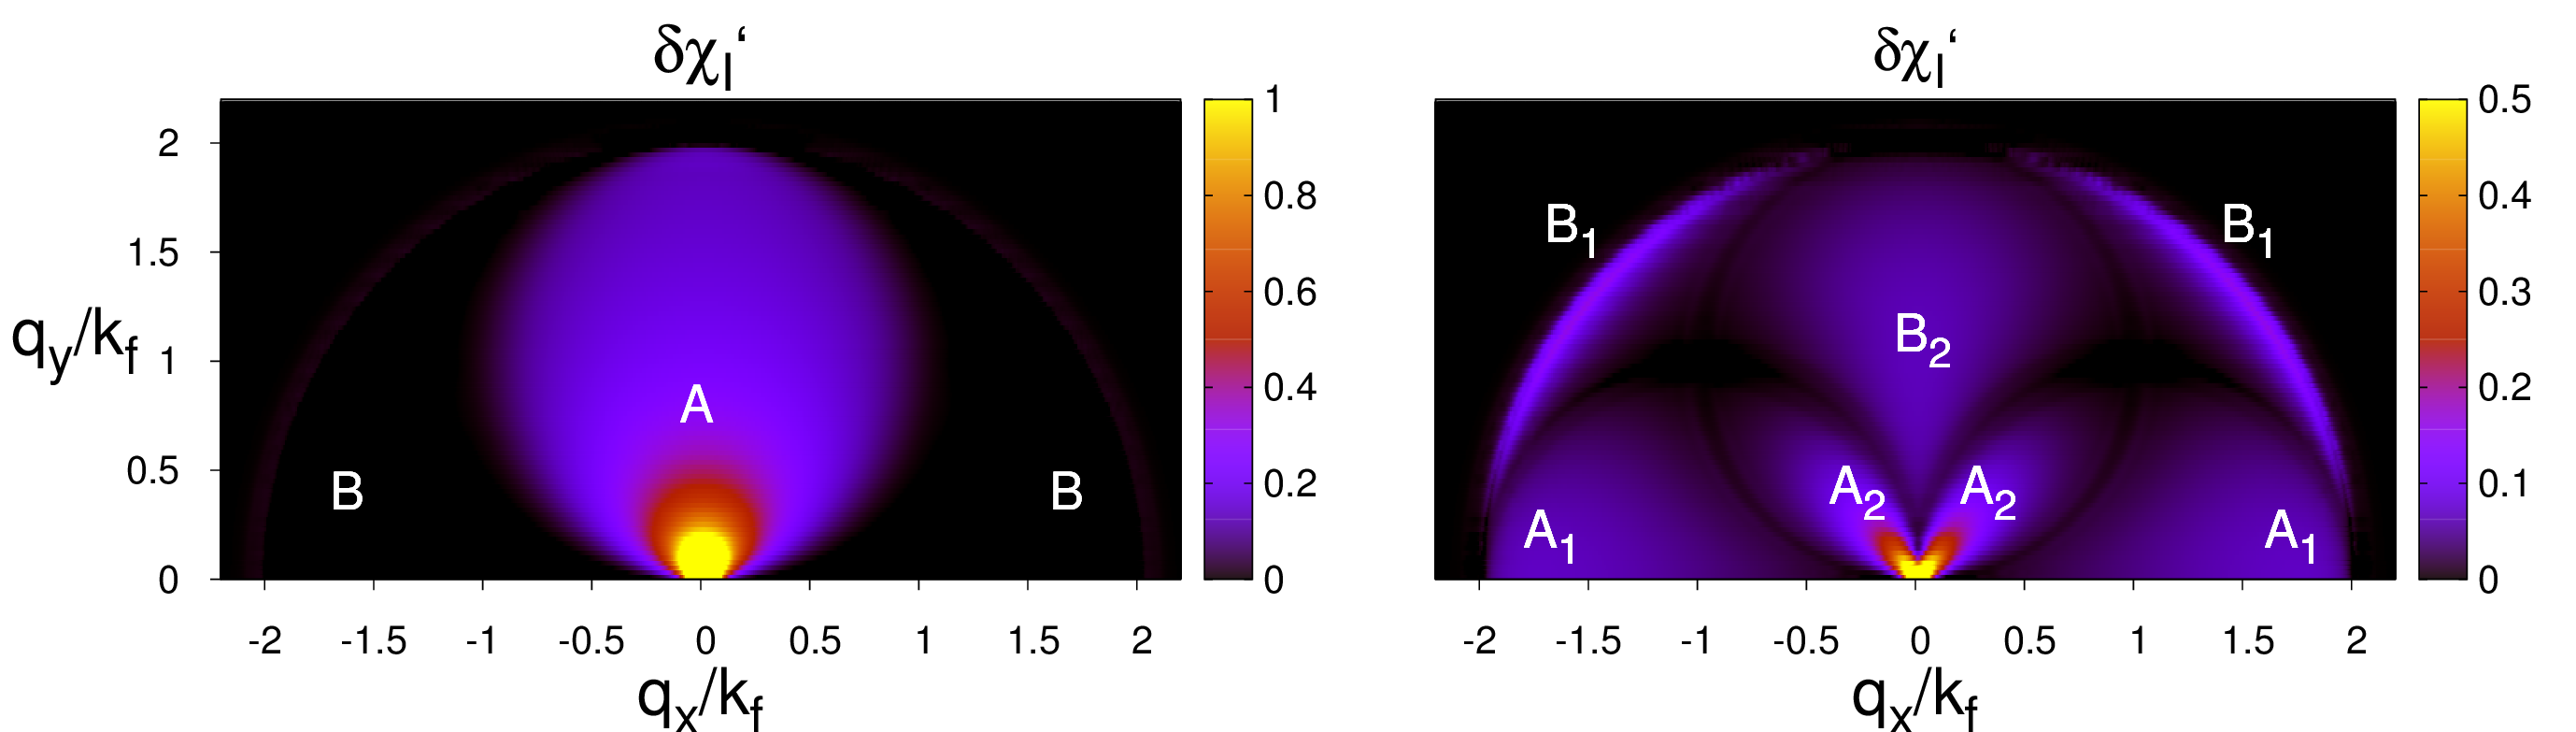
\includegraphics[scale=0.08]{./figures_3/fig2_SD_andreev/Fig2_andreev_cut.png}\\
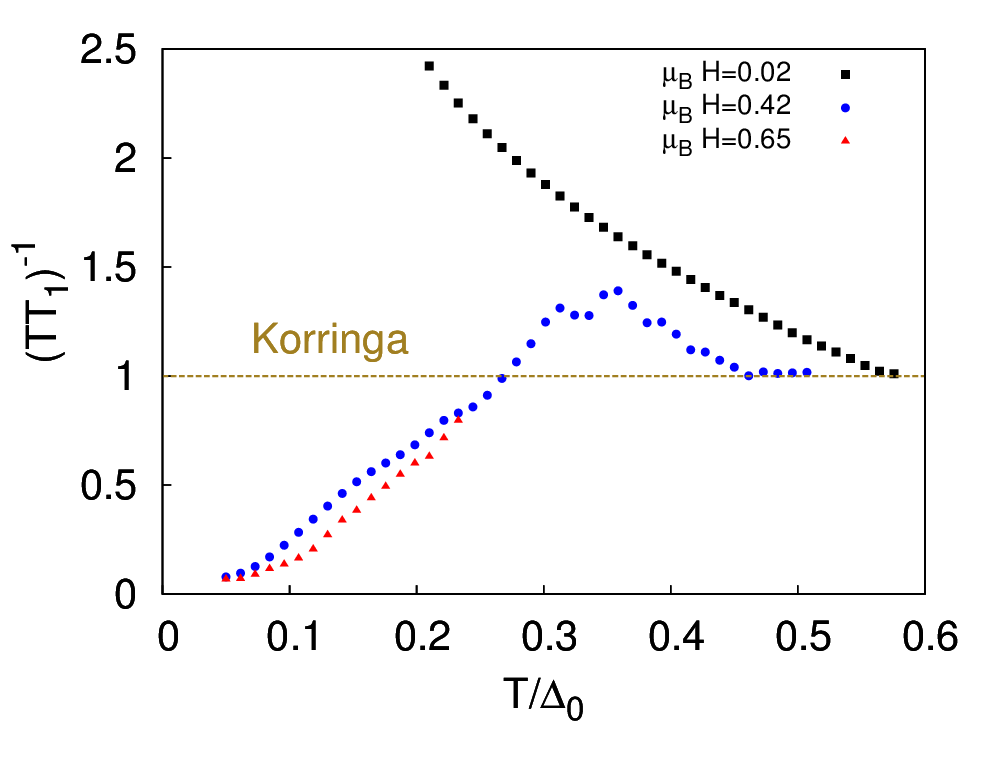
\includegraphics[scale=0.11]{./figures_3/fig_5/Fig5S_2.png} 
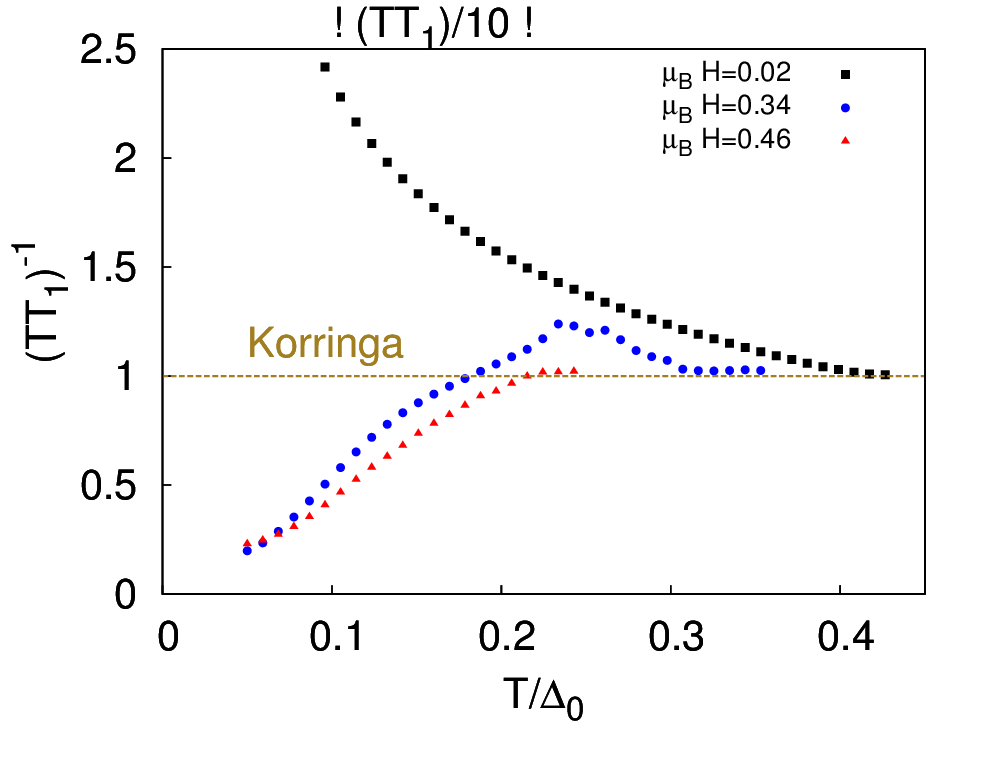
\includegraphics[scale=0.11]{./figures_3/fig_5/Fig5D_2.png}
\end{column}
\end{columns}
\end{frame}

%%%%%%%%%%%%%%%%%%%%%%%%%%%%%%%%%%%%%%%%%%%%%%%%%%%%%%%%%%%%%%%%%%%%%%%%%%%%%%%%%%%%%%%%%%%%%%%%%%%%%%%%%%%%%%%%%%%%%%%%%%%%
%%%%%%%%%%%%%%%%%%%%%%%%%%%%%%%%%%%%%%%%%%%%%%%%%%%%%%%%%%%%%%%%%%%%%%%%%%%%%%%%%%%%%%%%%%%%%%%%%%%%%%%%%%%%%%%%%%%%%%%%%%%%
%%%%%%%%%%%%%%%%%%%%%%%%%%%%%%%%%%%%%%%%%%%%%%%%%%%%%%%%%%%%%%%%%%%%%%%%%%%%%%%%%%%%%%%%%%%%%%%%%%%%%%%%%%%%%%%%%%%%%%%%%%%%

\end{document}